\documentclass[a4paper, 11pt]{tubsreprt}
\usepackage[ngerman]{babel}
\usepackage[utf8]{inputenc}
\usepackage{cite}
\usepackage{graphicx}
\usepackage{wrapfig}
\usepackage{subfigure}
\usepackage{hyperref}
\title{Wärmebehandlung}
\date{Wintersemester 17/18}
\author{J. Hansen, S. Vodde,
 J. Veer, T. Stein}

\logo{
	
\includegraphics{Bilder/ifw-logo.jpg}
}

\begin{document}
\maketitle
\tableofcontents
\chapter{Titanwerkstoffe}
Dieses Kapitel behandelt die für Titan charakteristischen Eigenschaften. Es wird vorerst auf generelle Eigenschaften eingegangen und dann die der Legierung Ti-6Al-4V. Gefügemerkmale, intermetallische Verbindungen und die Eigenschaften der einzelnen Legierungselemente sind Teil dieses Kapitels.
\section{Gefügemerkmale}\label{Abschnitt Gefügemerkmale}
Wie andere Metalle liegt Titan in verschiedenen Gittermodifikationen beziehungsweise Phasenzuständen vor. Der Zustand ist von der Temperatur und den vorliegenden Legierungselementen abhängig. Bei reinem Titan liegt zwischen 1668°C und 882°C ein kubisch raumzentriertes Kristallgitter vor. Diese Phase wird als Beta-Phase ($\beta$-Phase) bezeichnet. Bei 882°C erfährt Titan eine Phasenumwandlung zu einem hexagonalen Gitter. Diese Phasenumwandlungstemperatur wird als Betatransus-Temperatur bezeichnet und ist für jede Legierung unterschiedlich, denn die Legierungselemente haben Einfluss auf diese Temperatur. \cite{Luetjering2007}.

Das hexagonale Gitter wird als Alpha-Phase ($\alpha$-Phase) bezeichnet. Wenn das Material langsam abgekühlt ist, liegt reines Titan bei Raumtemperatur nahezu vollständig als Alpha-Phase vor. 

Dieses Gitter ist annähernd am dichtesten gepackt. Das Verhältnis in der Zelle ist etwas kleiner, als das in der ideal am dichtesten gepackten Zelle, c:a von Alpha-Titan liegt bei 1.586, wobei c und a die Längen innerhalb einer Zelle sind. Die perfekte hexagonale Zelle hat ein Verhältnis von 1.624 \cite{Luetjering2007}. Je nach Aufbau der Zelle sind diese Längen unterschiedlich groß.

Die Phasenumwandlung zwischen Beta- und Alpha-Phase kann auch martensitisch erfolgen. Dabei muss das Material aus einer ausreichend hohen Temperatur abgeschreckt werden. Diese Temperatur wird als Martensitstart-Temperatur bezeichnet. Sie ist wie die Betatransus-Temperatur von den Legierungselementen abhängig.  

\subsection{Alpha-Phase}
Die Alpha-Titan Phase ist durch eine hexagonale Gitterstruktur gekennzeichnet. Dadurch entsteht ein anisotropes Werkstoffverhalten in einem Korn beziehungsweise Einkristall.
Ein Einkristall ist über ein homogenes, einheitliches Kristallgitter definiert.
In einem Belastungsfall dieses Einkristalls ist das Werkstoffverhalten abhängig von der Belastungsrichtung im Verhältnis zur Gitterrichtung. Eine Kenngröße, die das elastische Verhalten eines Werkstoffes definiert, ist das Elastizitätsmodul: 
\begin{equation}
E=\sigma*\epsilon
\end{equation}
Das Elastizitätsmodul ist das Verhältnis zwischen der anliegenden Spannung $\sigma$ und die dadurch resultierende Dehnung $\epsilon$.
Es wird in Pascal angegeben. Das Elastizitätsmodul $E$ reicht je nach Verhältnis von minimal 100 GPa bis maximal 145 GPa. 

Allerdings wird Titan sehr selten als Einkristall hergestellt, sodass die unterschiedliche Kornorientierung dafür sorgt, dass die Anisotropie der einzelnen Körner sich gegenseitig aufhebt. Somit kann man von einem isotropen Werkstoffverhalten ausgehen.


\subsection{Beta-Phase}
Eine Beta-Phase ist ein Gefüge mit einer kubisch raumzentrierten Gitteranordnung. Daraus resultiert ein homogenes Werkstoffverhalten.

Eine große Menge an Beta-Phase existiert in der Regel bei Raumtemperatur nur unter bestimmten Bedingungen. Sie kann als metastabile Phase auftreten, was bedeutet, dass das Material nicht vollständig den Phasenübergang abschließen konnte und so in dem Zustand aus höheren Temperaturen verblieben ist.  

Durch Zusatz bestimmter Legierungselemente kann die $\beta$-Phase auch in größeren Mengen vorliegen. Dies wird im Kapitel ''betastabilisierende Legierungselemente'' näher erläutert.
\section{Gefüge}



Ausgehend von grundlegend verschiedenen Gefügen können diese durch Wärmebehandlung hinsichtlich ihrer mechanischen Eingenschaften optimiert werden. Eine Kombination aus mehreren Gefügeausprägungen können die Vorteile der einzelnen kombinieren. Dazu werden mehrstufige Wärmebehandlungen eingesetzt. Die Proben, die in dieser Arbeit verwendet werden, können nicht mehr rekristallisiert werden, sodass die verbleibenden Wärmebehandlungen auf Parameter wie Korngröße kaum Einfluss nehmen können. Das Gefüge ist somit von dem Ausgangsgefüge abhängig.  
\subsection{Lamellar}
Lamellare Gefüge sind unabhängig von dem Ausgangsgefüge einstellbar. Sie entstehen aus einer Abkühlung aus dem $\beta$-Gebiet. Während des Abkühlens bilden sich in den Korngrenzen der $\beta$-Phase $\alpha$-Bereiche, die in das $\beta$-Korn hinein wachsen. Die Alphabereiche wachsen erst in eine Richtung bevor sie ihre Dicke erhöhen. Je nach Abkühlgeschwindigkeit entstehen so dünne oder dickere Nadeln. Die Abbildung 1.1 zeigt ein beispielhaftes Gefüge, indem voll lamellare Strukturen zu sehen sind. Lamellare Gefüge werden auch als Widmannstättengefüge bezeichnet \cite{Luetjering2007}.


\begin{figure}
	\centering
		\includegraphics[scale=1]{Bilder/lamellar.jpg}
		\captionof{figure}[lamellares Gefüge]{Volllamellares Gefüge \cite{Leyens2002}}
		\label{lamellar}
		
\end{figure}
\subsection{Martensit}
Der Martensit ist eine metastabile Phase, die unter bestimmten Umständen entstehen kann. Aufgrund von Diffusionsvorgängen während eines Glühvorganges verändert sich der Anteil an Legierungselementen innerhalb einer Phase. Dem entsprechend reichert sich die Betaphase mit Beta stabilisierenden Legierungselementen an. Ist diese Anreicherung zu groß, kann eine martensitische Umwandlung der Betaphase nicht statt finden. Um diese Anreicherung zu regulieren, kann die Temperatur verwendet werden. Für eine Martensitbildung muss die Temperatur oberhalb der so genannten Martensitstart Temperatur liegen. Bei dieser wird eine zu große Anreicherung vermieden, da die Betaphase bei steigendem Volumenanteil eine geringere Konzentration an Beta stabilisierenden Legierungslementen besitzt. Die Martensitstart Temperatur sinkt, je höher die Konzentration an Beta stabilisierenden Elemente in der Phase ist, sodass sie unterhalb der Raumtemperatur liegen kann. Dann ist ein Erzeugen des martensitischen Gefüges nicht mehr möglich.

Neben der Glühtemperatur ist auch die Abkühlgeschwindigkeit entscheidend. Diffusionsvorgänge, die bei einer langsamen Abkühlung stattfinden, finden bei einer martensitischen Umwandlung nicht statt, da Abkühlgeschwindigkeiten von über 500 K/s durch eine Wasserabschreckung vorherschen. Aufgrund der unterschiedlichen Gitterstrukturen der Alpha- und Betaphase kommt es so zu einem scherartigen, diffusionslosen Umklappvorgang von einem kubisch raumzentrierten Gitter zu einem hexagonalen Gitter. Anders als bei Stahl kommt es nur zu einer minimalen Gitterverzerrung, da es keine zwangsgelösten Elemente in der Martensit-Phase gibt, die eine Gitterverzerrung verursachen würden. Die entstehende Verzerrung resultiert ausschließlich aus der Umwandlung des Gitter. Das hexagonale Gitter besitzt eine andere Raumausdehnung als das kubisch raumzentrierte Gitter. Durch den Umklappvorgang wandelt sich das Gitter bei konstantem Volumen. Daraus resultiert eine geringe Verzerrung des Gitters \cite{Luetjering2007}. Das charakteristische Martensitgefüge wie in Abbildung \ref{vollmartensit} resultiert aus dem Umwandlungsvorgang. Wie bei lamellaren Strukturen entstehen ausgehend von den ehemaligen Korngrenzen des Betakorns Nadeln, die in das Korn hinein wachsen. Im Gegensatz zu lamellaren Gefügen sind die Nadeln im Martensit wesentlich feiner \cite{Luetjering2007}.

Liegt eine bestimmte Konzentration an Beta stabilisierenden Elemente vor, verzerren diese metastabil geslösten Elemente das Kristallgitter und es kommt zu einem eher orthorhombischen Gitter. Die ehemalige hexagonale Struktur des Martensits wird auch als $\alpha'$ bezeichnet, das orthorhombrische Gitter als $\alpha''$ \cite{Luetjering2007}. 

\begin{figure}
\centering
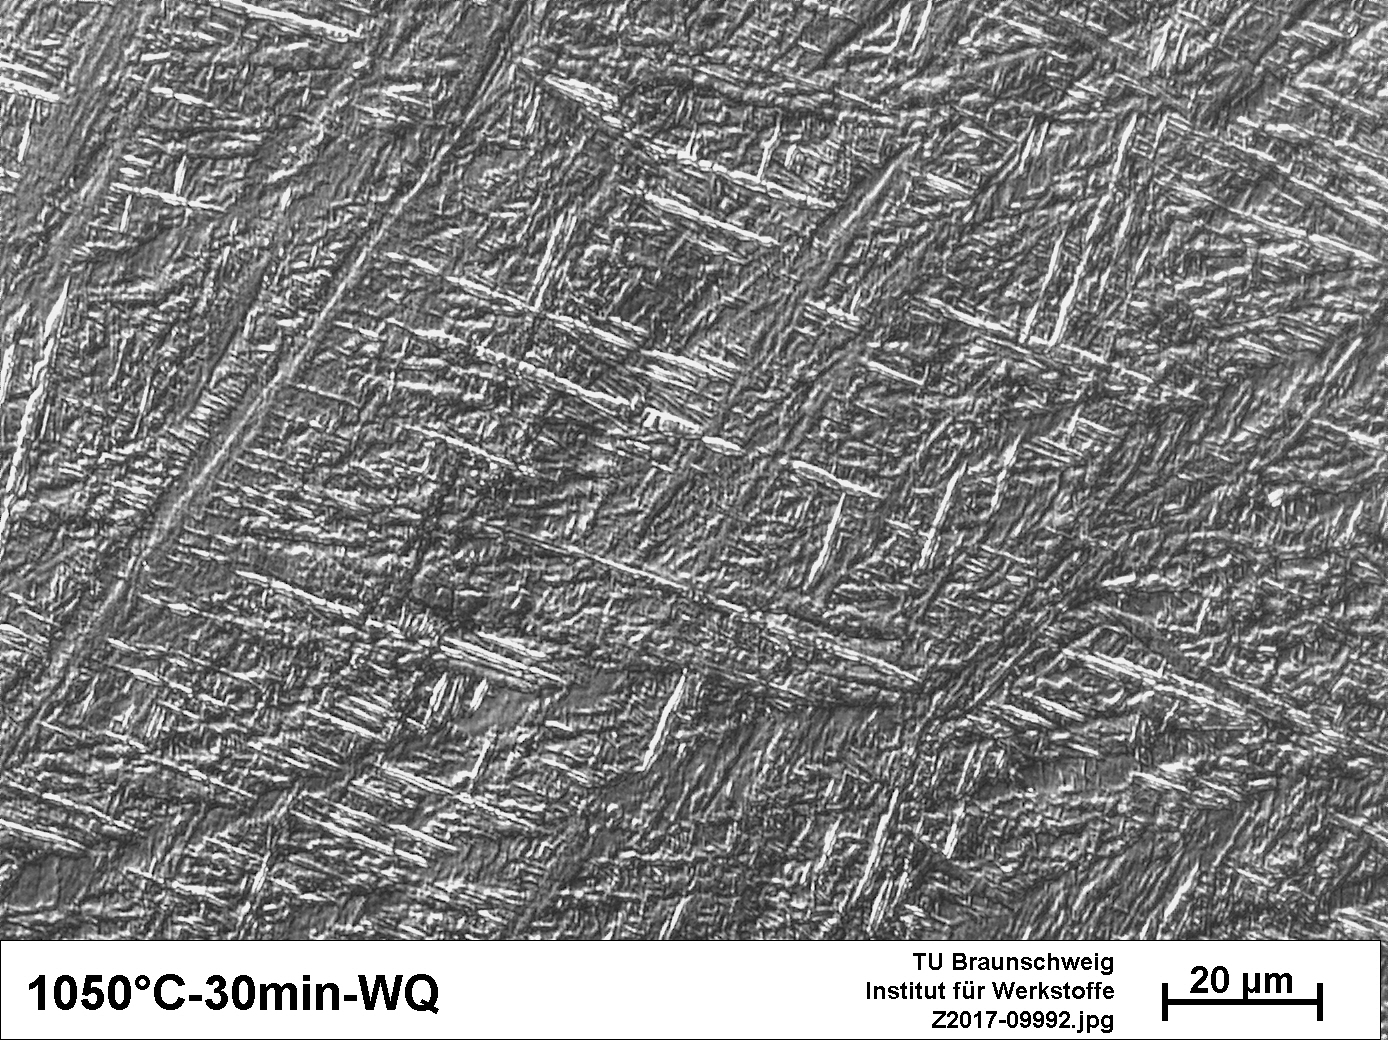
\includegraphics[width=0.4\textwidth]{Bilder/Vollmartensit.jpg}
\caption{Vollmartensitisches Gefüge}
\label{vollmartensit}
\end{figure}
\subsection{Globular}
Globulare Phase besteht aus runden Alpha-Bereichen. Dieses Gefüge resultiert aus einer Rekristallisation. Die Größe der einzelnen Körner ist von der Versetzungsdichte innerhalb des Gefüges vor der Rekristallisation abhängig. Nach einer Rekristallisation ist nur noch eine Zunahme der Korngröße realisierbar. Ausgehend aus diesem Gefüge lassen sich alle anderen Gefüge einstellen. In Abbildung \ref{globular} erkennt man ein solches Gefüge. 
\begin{figure} %Globulares Gefüge
\centering
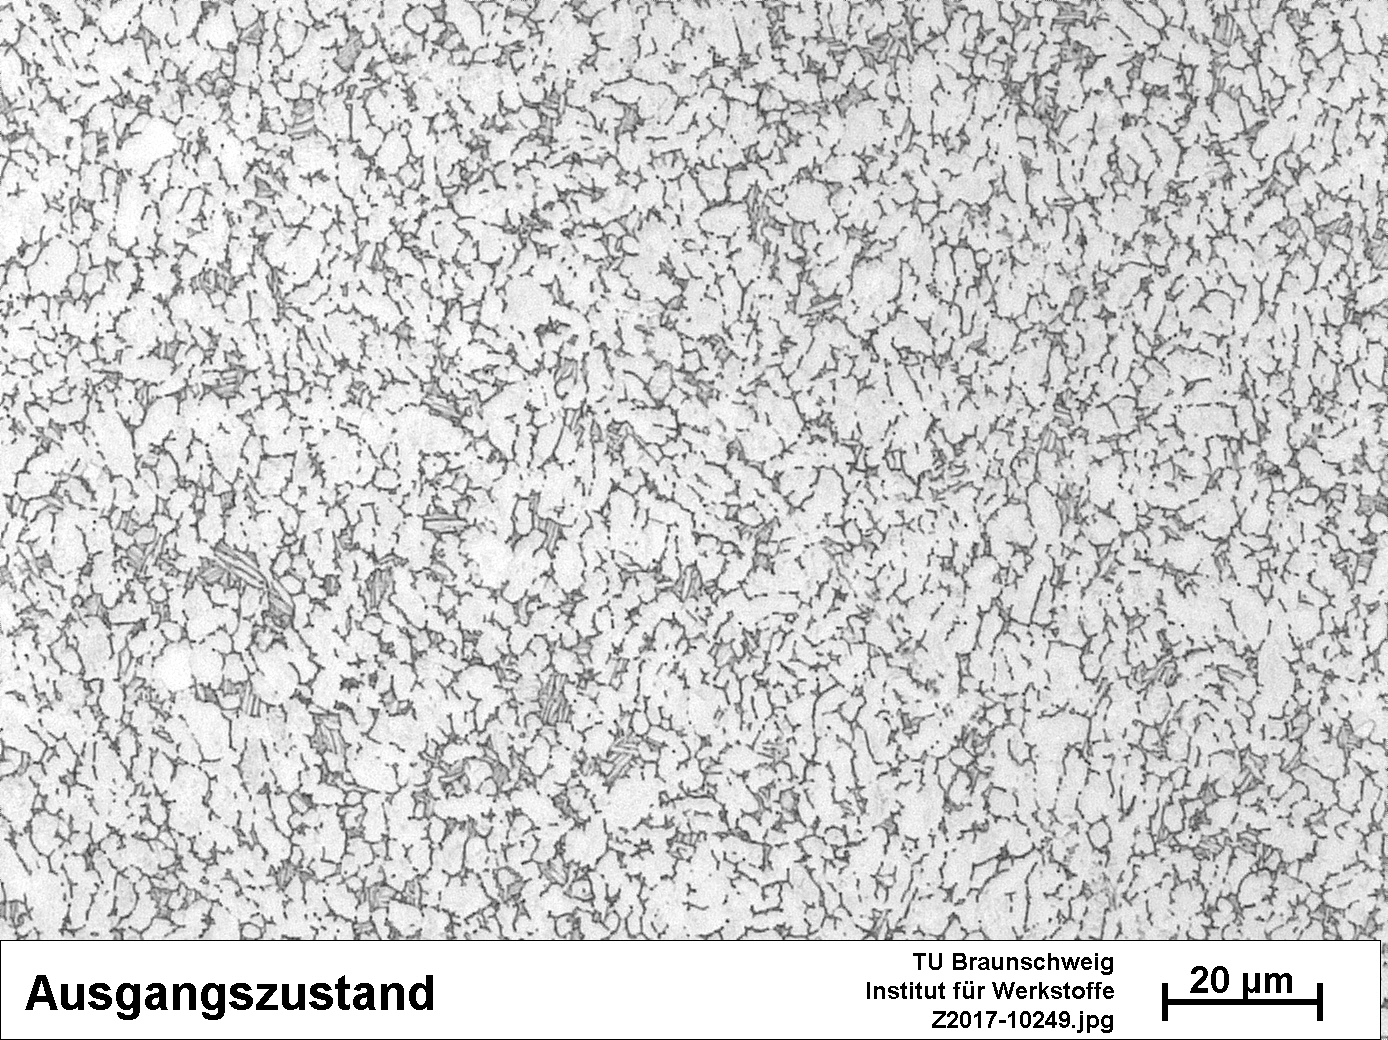
\includegraphics[width=0.4\textwidth]{Bilder/Ausgangsgefuege.jpg}
\caption{Globulares Gefüge}
\label{globular}
\end{figure}

\section{Intermetallische Verbindungen}
Titanlegierungen können, wie alle anderen Metalllegierungen, intermetallische Verbindungen bzw. Phasen bilden. Der Gittertyp der Phase passt meist nicht zu den Gittertypen der einzelnen Komponenten [vgl. Domke (1986)]. Abhängig vom Gittertyp der Grundmatrix und der Verbindung,  können kohärente, teilkohärente oder inkohärente Verbindungen entstehen. Die Grenzflächenenergie der kohärenten Teilchen ist gering. Sie verzerren das Kristallgitter nur etwas. Wachsen diese zu inkohärenten Teilchen heran, steigt die Grenzflächenenergie und das Kristallgitter wird stärker verzerrt.
Bestimmte Titanlegierungen nutzen diese intermetallischen Phasen, um die mechanischen Eigenschaften auch bei höheren Temperaturen zu Verbesseren [vgl. G.Lütjering, J.C. Williams 2007].   
Reines Titan kann keine intermetallischen Phasen bilden. Ausschlaggebend hierfür sind die Legierungselemete, die Alpha und Beta Stabilisatoren.  Diese Phasen lassen sich wie die Stabilisatoren  in Alpha und Beta Phasen aufteilen.  

\subsection{Alpha-Phasen}
Mit steigendem Aluminium Äquivalent können sich intermetallische Titan-Aluminium-Phasen bilden, die bei Raumtemperatur beständig sind. Wie das Diagramm ……….. zeigt, beginnt dieser Vorgang bereits bei ca. 5 \% Aluminium. Das zwei Phasen Gebiet $\alpha$Ti und Ti3Al bildet sich. Für die meisten Titanlegierungen gilt jedoch der Richtwert von 6 \% Aluminium um Ti3Al ($\alpha$2) Teilchen auszuscheiden.  Die Ti3Al Teilchen besitzen eine hexagonale Gitterstruktur wie das $\alpha$Ti. Die Teilchen können  die gleichen Gitterplätze besetzten und verzerren das Kristallgitter nur wenig. Sie sind kohärent.
Werden noch größere Anteile Aluminium  zum Titan legiert, kann sich TIAl ( $\gamma$-TiAl) bilden. Diese Teilchen besitzen ein Tetragonales Kristallgitter.
 Werden Legierungen mit diesen beiden genannten Phasen erzeugt, entstehen sogenannte Titan-Aluminide \cite{Luetjering2007}.   
\begin{figure}
\centering
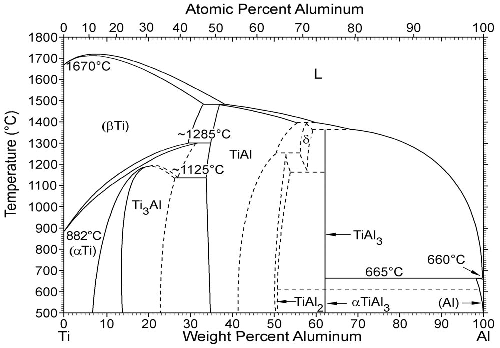
\includegraphics[width=0.5\textwidth]{Bilder/Titanaluminide.png}
\caption{Titan Aluminium Phasendiagramm}
\end{figure}
 
\subsection{Beta-Phasen}
Intermetallische Beta-Phasen sind in Titanlegierungen unerwünscht, da sie die mechanischen Eigenschaften verschlechtern. Die isomorphen Stabilisatoren, wie Molybdän, Vanadium oder Niob, bilden in gewöhnlichen Legierungen keine intermetallischen Phasen. Ihre Legierungsanteile sind zu gering. Die eutektoiden Stabilisatoren, wie Chrom oder Eisen hingegen, bilden diese. TiFe und Ti$_{2}$Cr Phasen sollen in Titanlegierungen nicht entstehen \cite{Luetjering2007}.
\section{Ti-6Al-4V}
Im Mittelpunkt der in dieser Arbeit behandelten Aufgabenstellung steht der Werkstoff Titan mit den Legierungszusätzen von sechs Gewichtsprozent Aluminium und vier Gewichtsprozent Vanadium. Anders ausgedrückt: Titan-6Al-4V. Im Folgenden soll demnach ein wenig näher auf die Eigenschaften dieser Legierung eingegangen werden. 
\subsection{Legierungselemente und Verwendung}
Titan 6 Aluminium 4 Vanadium oder kurz Ti-64 ist die am häufigsten verwendete Titanlegierung weltweit. Sie wurde bereits in den 1950er Jahren entwickelt und zählt zu den am besten erforschten Titanlegierungen \cite{Leyens2002}. Wegen ihrer großen Bedeutung in der Luftfahrt, werden Titanlegierungen häufig auch in anderen Bereichen der Technik nach den in der Luftfahrt geltenden Normen bestellt. Ein Blick auf die AMS 4911 (aerospace material specification) offenbar hier die Vorgaben für die chemische Zusammensetzung der Legierung. Neben den bereits im Namen Ti-64 festgelegten 6\% Aluminium und 4\% Vanadium sind bis zu 0,25\% Eisen und 0,2\% Sauerstoff als Legierungselemente zugelassen. Durch seine Legierungselemente Aluminium als Stabilisator der Alpha-Phase und Vanadium als Beta-stabilisierendes Element, lässt sich Ti-64 zu den Alpha+Beta Legierungen zählen.
Die Hauptverwendung der Legierung liegt wie oben bereits erwähnt in der Luftfahrt. Hier kommt sie zum Beispiel als Material für Schaufeln im Fan und Niederdruckverdichter vor \cite{Luetjering2007}[S.250 ff]. Weiter findet man Anwendungen in der Medizintechnik. Hier werden gerade Implantate von denen eine etwas höhere Festigkeit verlangt wird nicht mehr aus commercially pure (CP) Titan sondern aus Ti-64 hergestellt. Da ist insbesondere bei Hüftimplantaten oder Schrauben der fall \cite{Luetjering2007}[S. 400 f.]

\subsection{Mechanische Eigenschaften}
Die mechanischen Eigenschaften von Ti-64 hängen wie bei anderen Legierungen des Basiswerkstoffes Titans auch von der abschließenden Wärmebehandlung ab. In Abhängigkeit der durchgeführten Wärmebehandlung schwanken die Angaben in der Literatur. Die Beta-Transus-Temperatur bildet einen zentralen Bezugspunkt für die Einstellung eines Gefüges und liegt für Ti-64 zwischen 985°C und 1000°C. Sie wird meist mit 995°C angegeben \cite{Semiatin2003}, \cite{Chen2008}. Durch seine Legierungselemente ist Ti-64 in der Lage bei Raumtemperatur sowohl in Alpha- als auch Beta-Phase aufzutreten.
Ein mögliches Gefüge stellt hierbei das Bi-modal- oder Duplexgefüge da. In Kombination mit einem bis über 200 Stunden andauerndem Auslagern lässt sich hier zusätzlich eine Ausscheidung von Titan3-Aluminium herbeiführen. Dieses Gefüge verbessert gerade die, aufgrund der geringen Wärmeleitfähigkeit, schlechten Impact-Eigenschaften von Ti-64 \cite{Semiatin2003}.
Ein weiteres mögliches Gefüge stellt das lamellare Gefüge dar. Als lamellare Gefüge versteht man Widmannstätten- oder martensitische-Gefüge. Die Festigkeit hängt hier maßgeblich von der Größe paralleler lamellarer Bereiche und der Alpha-Lamellenbreite ab. Eine geringe Alpha-Lamellenbreite von 3 Mikrometern verspricht hierbei für Ti-64 eine optimale Festigkeit \cite{Sieniawski2013}. Einstellen lassen sich lamellare Gefüge durch ein langsames Abkühlen (Widmannstätten) oder Abschrecken (martensitisch) von oberhalb der Beta-Transus-Temperatur. 
Die Aufgabenstellung dieser Arbeit sieht vor die Zugfestigkeit von Ti-64 in Hinblick auf eine Verwendung als Triebwerksmaterial zu optimieren. Möglichst hohe Festigkeiten lassen sich dabei mit beiden oben aufgezeigten Gefügen erreichen. Einen Überblick gibt Tabelle [Tabellennummer]
\subsection{Bi-Modal}
Bi-Modal-Gefüge (Duplex-Gefüge) sind durch globularer $\alpha$-Phase und Lamellen aus $\alpha$- und $\beta$-Phase gekennzeichnet. Es resultiert meist aus einer geglühten Probe.  In Abbildung \ref{bimodal} ist ein solches Gefüge zu erkennen. 
\begin{figure}
\centering
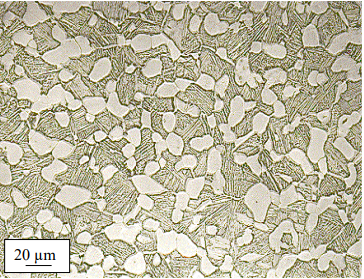
\includegraphics[width=0.4\textwidth]{Bilder/Duplexgefuege.PNG}
\caption[Bi-Modal-Gefüge]{Bi-Modal-Gefüge\cite{Werkstoffdesign2012}}
\label{bimodal}
\end{figure}

\chapter{Methodik}
\section{Intermetallische Verbindung}
Titanlegierungen können, wie alle anderen Metalllegierungen, intermetallische Verbindungen bzw. Phasen bilden. Der Gittertyp der Phase passt meist nicht zu den Gittertypen der einzelnen Komponenten [vgl. Domke (1986)]. Abhängig vom Gittertyp der Grundmatrix und der Verbindung,  können kohärente, teilkohärente oder inkohärente Verbindungen entstehen. Die Grenzflächenenergie der kohärenten Teilchen ist gering. Sie verzerren das Kristallgitter nur etwas. Wachsen diese zu inkohärenten Teilchen heran, steigt die Grenzflächenenergie und das Kristallgitter wird stärker verzerrt.

Bestimmte Titanlegierungen nutzen diese intermetallischen Phasen, um die mechanischen Eigenschaften auch bei höheren Temperaturen zu Verbessern \cite{Luetjering2007}.

Reines Titan kann keine intermetallischen Phasen bilden. Ausschlaggebend hierfür sind die Legierungselemete, die $\alpha$- und $\beta$- Stabilisatoren.  Diese Phasen lassen sich wie die Stabilisatoren  in $\alpha$- und $\beta$- Phasen aufteilen.  
\subsection{Alpha-Phasen}
Mit steigendem Aluminium Äquivalent können sich intermetallische Titan-Aluminium-Phasen bilden, die bei Raumtemperatur beständig sind. Wie das Diagramm ……….. zeigt, beginnt dieser Vorgang bereits bei ca. 5 \% Aluminium. Das zwei Phasen Gebiet $alpha$Ti und Ti3Al bildet sich. Für die meisten Titanlegierungen gilt jedoch der Richtwert von 6 \% Aluminium um Ti3Al ($\alpha2$) Teilchen auszuscheiden.  Die Ti3Al Teilchen besitzen eine hexagonale Gitterstruktur wie das $\alpha$Ti. Die Teilchen können  die gleichen Gitterplätze besetzten und verzerren das Kristallgitter nur wenig. Sie sind kohärent.
Werden noch größere Anteile Aluminium  zum Titan legiert, kann sich TIAl ( $\gamma$-TiAl) bilden. Diese Teilchen besitzen ein Tetragonales Kristallgitter.
 Werden Legierungen mit diesen beiden genannten Phasen erzeugt, entstehen sogenannte Titan-Aluminide \cite[vgl.]{Luetjering2007}.   

\subsection{Beta-Phasen}
Intermetallische Beta-Phasen sind in Titanlegierungen unerwünscht, da sie die mechanischen Eigenschaften verschlechtern. Die isomorphen Stabilisatoren, wie Molybdän, Vanadium oder Niob, bilden in gewöhnlichen Legierungen keine intermetallischen Phasen. Ihre Legierungsanteile sind zu gering. Die eutektoiden Stabilisatoren, wie Chrom oder Eisen hingegen, bilden diese. TiFe und Ti2Cr Phasen sollen in Titanlegierungen nicht entstehen \cite{Luetjering2007}.

\section{Rasterelektronenmikroskopie}
Das Rasterelektronenmikroskop (REM) bietet eine bessere Auflösung und eine größere Vergrößerung, als das Auflichtmikroskop. Es können Vergrößerungen von bis 100000 x erreicht werden. Die Auflösung liegt bei wenigen Nanometer. Durch eingebaute Detektoren am REM können bestimmte analytische Methoden zusätzlich  durchgeführt werden. Dies ist hilfreich für Auswertung der Proben.
Eine Wolframdraht oder ein Lanthanhexaborideinkristall ($LaB_{6}$) dient als Elektronenquelle. Die Elektronen werden emittiert und mittels Beschleunigungsspannung in Richtung Anode abgelenkt. Je nach Auflösung kann die Spannung zwischen 200$V$ und 50$kV$ liegen. Elektromagnetische Linsen bündeln die Elektronen in einem Strahl und lenken ihn auf die Probe. Mit einer Anblenkspule kann der Strahl über die Probe geführt werden \ref{REM Aufbau}.

\begin{figure} %REM Aufbau
\centering
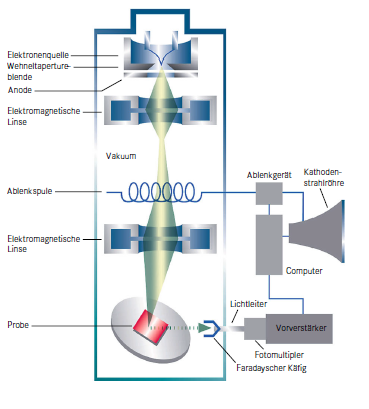
\includegraphics[width=0.5\textwidth]{Bilder/REM.png}
\caption{Aufbau eines Rasterelektronenmikroskops}
\label{REM Aufbau}
\end{figure}

Die Elektronen gelangen auf die Probeoberfläche und es entstehen Wechselwirkungen zwischen den Strahlelektronen und den Atomen der Probenoberfläche. Die zwei wichtigsten Erscheinungen sind hierbei die Rückstreuelektronen (RE) und die Sekundärelektronen (SE). Die Strahlelektronen werden durch die Atomkerne in der Probe abgelenkt  und verlieren an Energie. Diese Energie wird in Form der Röntgenbremsstrahlung frei. Die dabei teilweise zurückgeworfenen Elektronen werden als RE bezeichnet. Der Streuprozess zwischen den Strahlelektronen und den Elektronen in den Atomschalen, führt zu SE. Die hierbei entstehende Röntgenstrahlung, ist die charakteristische Röntgenstrahlung. Die Elektronen in den Atomschalen werden von den Strahlelektronen herausgeworfen. Die Schale ist ionisiert. Diese freien Plätze werden durch andere Elektronen besetzt. Die dabei freiwerdende Energie wird in Form von Röntgenstrahlung emittiert. Verlassen RE die Probe können zusätzlich SE entstehen.
Die SE und RE dienen nun der Bilderzeugung. Die Elektronen werden mit jeweils unterschiedlichen Detektoren erfasst. Die Spannung, die aus dem Detektorimpuls erzeugt wird, gelangt zur Kathodenstrahlröhre. Werden viele Elektronen erfasst, steigt die Spannung und der Bildpunkt erscheint hell. Die einzelnen Bildpunkte werden nun durch das „abrastern“ der Oberfläche erzeugt. Heutzutage erfolgt die Bildherstellung digital. [vgl. Romeis Mikroskopische Technik (2015)].
Gute Bildergebnisse können nur durch eine sorgfältige Probepräparation entstehen. Die Oberflächen müssen sauber sein. Die Proben sollten vor der Analyse im Ultraschallbad gereinigt werden.  Zudem muss die gesamte Probe elektrisch leiten. Eingebettete Proben können nicht verwendet werden. Der Kunststoff nimmt die Elektronen auf und würde den Elektronenstrahl ablenken. Als alternative kann eine leitende Gold oder Silberschicht aufgebracht werden.
\section{Wärmebehandlung}

Die Wärmebehandlung nach der Rekristallisation ist die letzte Methode, um das Gefüge des Titans einzustellen. Hierbei kommt es auf Parameter wie Temperatur, Haltezeit und Abkühlmethode an. Um die bereits erwähnten Gefüge zu realisieren, ist eine spezifische Abfolge von einer beziehungsweise mehreren Stufen einer Wärmebehandlung nötig. Die grundlegenden Behandlungen werden in diesem Kapitel behandelt, die speziellen, mehrstufigen, soweit relevant, im dritten.
\subsection{Temperaturkontrolle}
Für die Temperaturkontrolle innerhalb der Wärmebehandlung kommt ein Ofen zum Einsatz. Dieser kann bis zu Temperaturen deutlich oberhalb der Betatransus Temperatur aufheizen und diese mit einer Genauigkeit von drei Kelvin halten. So kann der Temperaturbereich, der für die Wärmebehandlungen wichtig ist, eingestellt werden. Dieser liegt zwischen Raumtemperatur und 50°C - 100°C oberhalb der Betatransus Temperatur. Der Ofen ist außerdem für die insoweit bedeutende Aufheizgeschwindigkeit verantwortlich.

\subsection{Abkühlmedien}

Durch Abkühlmedien werden bestimmte Abkühlgeschwindigkeiten realisiert. Für langsamere Abkühlungen als in der Luft wird der Ofen genutzt. Hier kann die Temperatur beliebig langsam reduziert werden. Ein weiterer Vorteil des Ofens ist, dass die Probe auf eine bestimmte Temperatur herunter gekühlt werden kann. Dies ist für mehrstufige Wärmebehandlungen wichtig, bei denen eine Abkühlung auf Raumtemperatur zwischen den Schritten vermieden werden soll. 

Da der Ofen nicht überaus schnell abkühlen kann, wird zur schnelleren Abkühlung Luft mit Raumtemperatur verwendet. Durch den höheren Temperaturgradienten im Verhältnis zum Ofen wird so die Abkühlung beschleunigt.  

Um noch schnellere Abkühlungen zu realisieren, wird Wasser oder Öl verwendet. So werden zum Beispiel Abkühlgeschwindigkeiten für eine Martensitbildung ermöglicht.
\section{Anpassung der Gefüge durch Wärmebehandlung}

\begin{figure}
	\centering
	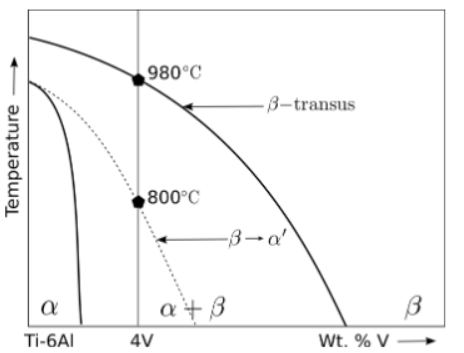
\includegraphics[width=0.5\textwidth]{Bilder/Phasendiagram.PNG}
	\caption[Phasendiagramm]{schematisches Phasendiagramm Ti-6Al-4V \cite{Babu2008}}
	\label{Phasendiagram}
\end{figure}
Das Anpassen der Gefüge ist das Ziel jeder Wärmebehandlungen. So werden Werkstoffeigenschaften gezielt für den jeweiligen Anwendungsfall optimiert, denn bestimmte Gefüge, mit bestimmten Mechanische Eigenschaften, folgen aus bestimmten Wärmebehandlungen. Diese Einstellung hat bestimmte Grenzen. Korngrößenreduzierung ist nicht möglich, sodass eine Behandlung mit Kornwachstum nicht Rückgängig gemacht werden kann. Eine derartige Behandlung sollte somit mit bedacht Gewählt werden, da gewöhnlich die Festigkeit durch Kornwachstum abnimmt.
\subsection{Lamellar}
Rein lamellare Strukturen folgen aus einer Abkühlung aus dem Beta-Gebiet. In dem Phasendiagramm aus Abbildung \ref{Phasendiagram} ist erkennbar, dass oberhalb der Betatransus Linie das Material in einem Einphasenfeld liegt und somit bei einer moderaten Abkühlung vollständig in lamellare Phase umwandelt. Wird die Glühtemperatur unterhalb der Betatransus Temperatur gewählt, ist das Material in einem Zweiphasengebiet. So können unterschiedliche Alphagehalte eingestellt werden, sodass eine Kombination aus Alpha-Phase und Alpha+Beta-Phase entsteht. Das so eingestellte Alpha-Gefüge wird auch als Primäralpha bezeichnet. 


Je nach Feinheit der Platten hat das Gefüge positive oder negative Eigenschaften bezüglich der Festigkeit. Fein lamellare Platten sorgen für eine Zunahme der Festigkeit und grobe Platten für eine Abnahme. Dies ist durch die unterschiedliche Grenzflächendichte zu erklären, denn die hohe Anzahl an Körnern behindert den Versetzungsfortschritt. Bei großen lamellaren Platten ist es für die Versetzung deutlich einfacher, durch das Bauteil zu wandern. 

\subsection{Martensit}
Martensit entsteht mit Glühtemperaturen höher als die Martensitstart-Temperatur, folgend aus einer Wasserabschreckung. Wie bei lamellaren Gefügen kann auch eine Kombination aus Primärem Alpha und Martensit erfolgen, indem die Glühtemperatur im 2-Phasengebiet gewählt wird. Wie hoch die Temperatur gewählt wird, entscheidet über den Primäralpha-Phasenanteil.

\subsection{Bi-Modal}
Diese Strukturen bestehen aus einer Kombination von Primär-Alpha und lamellaren Strukturen aus Alpha und Beta in den ehemaligen Betakörnern. Dies lässt sich durch eine Wärmebehandlung einstellen, in der die Glühungstemperatur unterhalb der Betatransus-Temperatur liegt. Die Temperatur entscheidet über die Ausprägung der primären Alphakörner. Aus dem Phasendiagramm aus Abbildung \ref{Phasendiagram} erklärt sich, dass, je höher die Glühungstemperatur ist, desto geringer ist der primäralpha-Gehalt in dem resultierenden Gefüge. Die Abkühlgeschwindigkeit entscheidet über die Breite der während des Abkühlvorgangs entstehenden Lamellen \cite{Luetjering2007}.

\subsection{Globular}
Wie in Kapitel eins bereits erwähnt, lässt sich ein globulares Gefüge nur durch eine Rekristallisierung ermöglichen. Es ist hierbei wichtig, dass das Material langsam abgekühlt wird, sodass sich die Alphakörner bilden können, ohne das sich ein Bi-Modal Gefüge einstellt \cite{Luetjering2007}.

\section{Auswertung der Proben}
\subsection{Auszählverfahren}
Das Auszählverfahren ist ein manuelles Hilfsmittel um die Phasenanteile von Gefügen zu ermitteln. Metalllegierungen, wie auch Titan, können unterschiedliche Gefüge mit mehreren Phasen ausbilden. Deren Anteile können mit diesem Verfahren bestimmt werden.

Das zu analysierende Gefüge wird mit einem Mikroskop abgebildet. Fünf zufällig ausgewählte Bildbereiche werden ausgedruckt und mit einem gleichmäßigen Raster versehen. Die Abbildung \ref{Raster für das Auszählverfahren} zeigt ein beispielhaftes Raster.
\begin{figure} %Raster für das Auszählverfahen
\centering
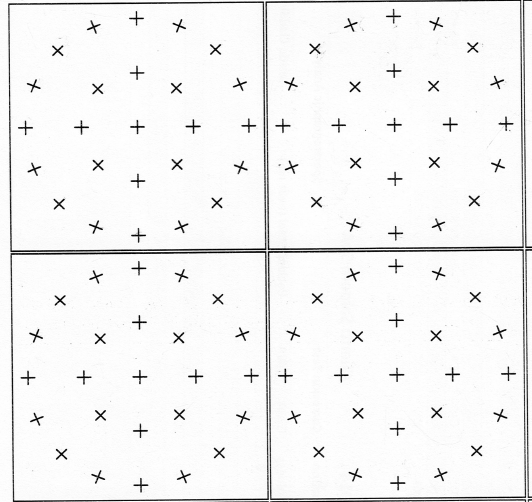
\includegraphics[width=0.5\textwidth]{Bilder/Raster.png}
\caption{Raster für das Auszählverfahren}
\label{Raster für das Auszählverfahren}
\end{figure}

Für eine gleichmäßige Verteilung der Phasen reichen die äußeren Ringe der Felder. Liegen die Anteile allerdings bei wenigen Prozent müssen alle Kreuze berücksichtigt werden. 
Anschließend erfolgt das Auszählen. Die Kreuze die auf der Phase liegen, die bestimmt werden soll, werden mit 1 gezählt. Liegen die Kreuze an einer Phasengrenze, werden sie mit 0,5 gezählt. Berühren die Kreuze die Phase nicht werden sie mit 0 gezählt. Alle Werte werden aufsummiert und durch die Anzahl aller gezählten Kreuze geteilt. Das Ergebnis ist der Phasenanteil. Dieses Verfahren wird an fünf unterschiedlichen Bildbereichen durchgeführt und der Mittelwert gebildet.

\subsection{Zugversuch}

Bei einem Zugversuch werden Proben bis zum Bruch gedehnt und dabei Werkstoffkennwerte bestimmt. Die Kennwerte sind unter anderem  Elastizitätsmodul, Elastizitätsgrenze, Zugfestigkeit und Bruchdehnung. Unter diesen Kennwerten ist für die Anforderung der Arbeit die Zugfestigkeit interessant, da diese über eine Wärmebehandlung optimiert werden soll. Sie ist die größte plastische Dehnung bevor sich das Bauteil einschnürt beziehungsweise reißt. Mit dem Zugversuch wird die Abschätzung der Zugfestigkeit über die Härte vermieden und es kann abgeschätzt werden, ob die Formel der Abschätzung realitätsnah war. Der Zugversuch wird mit einer Universalprüfmaschine der Firma Zwick Roell nach der Norm DIN EN ISO 6892-1 Teil B durchgeführt. Dabei werden die Zugproben nach DIN 50125-B5x25 angefertigt. Nach der Norm des Zugversuches wird die Spannungsgeschwindigkeit abhängig von dem Elastizitätsmodul des Werkstoffs gewählt. Da Titan ein E-Modul kleiner 150000 $MPa$ besitzt, wird eine Spannungsgeschwindigkeit zwischen 2 und 20 $MPa$~ $s^{-1}$ gewählt. Diese Spannungsgeschwindigkeit wird während der Bestimmung der Dehngrenze verwendet. Danach wird über eine Dehngeschwindigkeit von maximal $0,008$ $s^{-1}$ zur weiteren Messung benutzt. Form B der Zugproben sind nach Norm Rundproben mit Gewinde zur Einspannung. Der Zusatz ''5x25'' beschreibt die Maße der Probe. 5 ist dabei der Probendurchmesser und 25 die Anfangsmesslänge. 

\chapter{Wärmebehandlungen}
\section{Festigkeitssteigerung durch Martensitbildung}\label{Festigkeitssteigerung durch Martensitbildung}
Die Literaturrecherchen zeigen, dass sich die mechanischen Eigenschaften der Titanlegierung durch unterschiedliche Gefügestrukturen einstellen lassen. Die erste Methode um die Härte bzw. Zugfestigkeit zu steigern, ist die Einstellung des Primär Alpha Gehalts. Mit einem sinkenden Gehalt der Alpha Phase, steigt die Härte des Gefüges. \cite{Sahoo2015}. Der Alpha Anteil lässt sich mit einer Wärmebehandlung variieren. 
Mit einer Wärmebehandlung im zwei Phasen Gebiet ($\alpha'+ \beta$) sinkt der Anteil der Alpha Phase mit steigender Temperatur, bis die Beta Transustemperatur erreicht ist (siehe Abbildung \ref{Phasendiagram}). Um diesen Anteil beizubehalten muss die Temperatur eine bestimmte Zeit gehalten und anschließend schnell abgekühlt werden. Die Diffusionsvorgänge sollen so klein wie möglich gehalten werden. Neue Alpha Körner sollen nicht entstehen und die vorhandenen Körner sollen nicht auf Kosten der Beta Phase weiter wachsen. Oberhalb der Martensitstarttemperatur kann sich aus der Beta Phase je nach Abkühlmedium Martensit oder transformierte Beta Phase bilden.

\subsection{Abhängigkeit des Primär Alpha Anteils von der Glühtemperatur}
Drei Proben wurden bei jeweils bei 950°C, 960°C und 970°C für eine Stunde im Ofen geglüht und anschließend im Wasser abgeschreckt. Anschließend wurden die Proben präpariert. Die Abbildungen aus \ref{Alle Glühen} zeigen die lichtmikroskopischen Aufnahmen. Primär Alpha Körner liegen in einer Martensit Matrix. Die Alpha Körner wurden durch das Abschrecken eingefroren, und die Beta Phase ist komplett in den Martensit umgeklappt. Die unterschiedlichen Primär Alpha Anteile sind klar zu erkennen.

\begin{figure}
\subfigure[Gefüge bei einer Glühungstemperatur von 970°C]{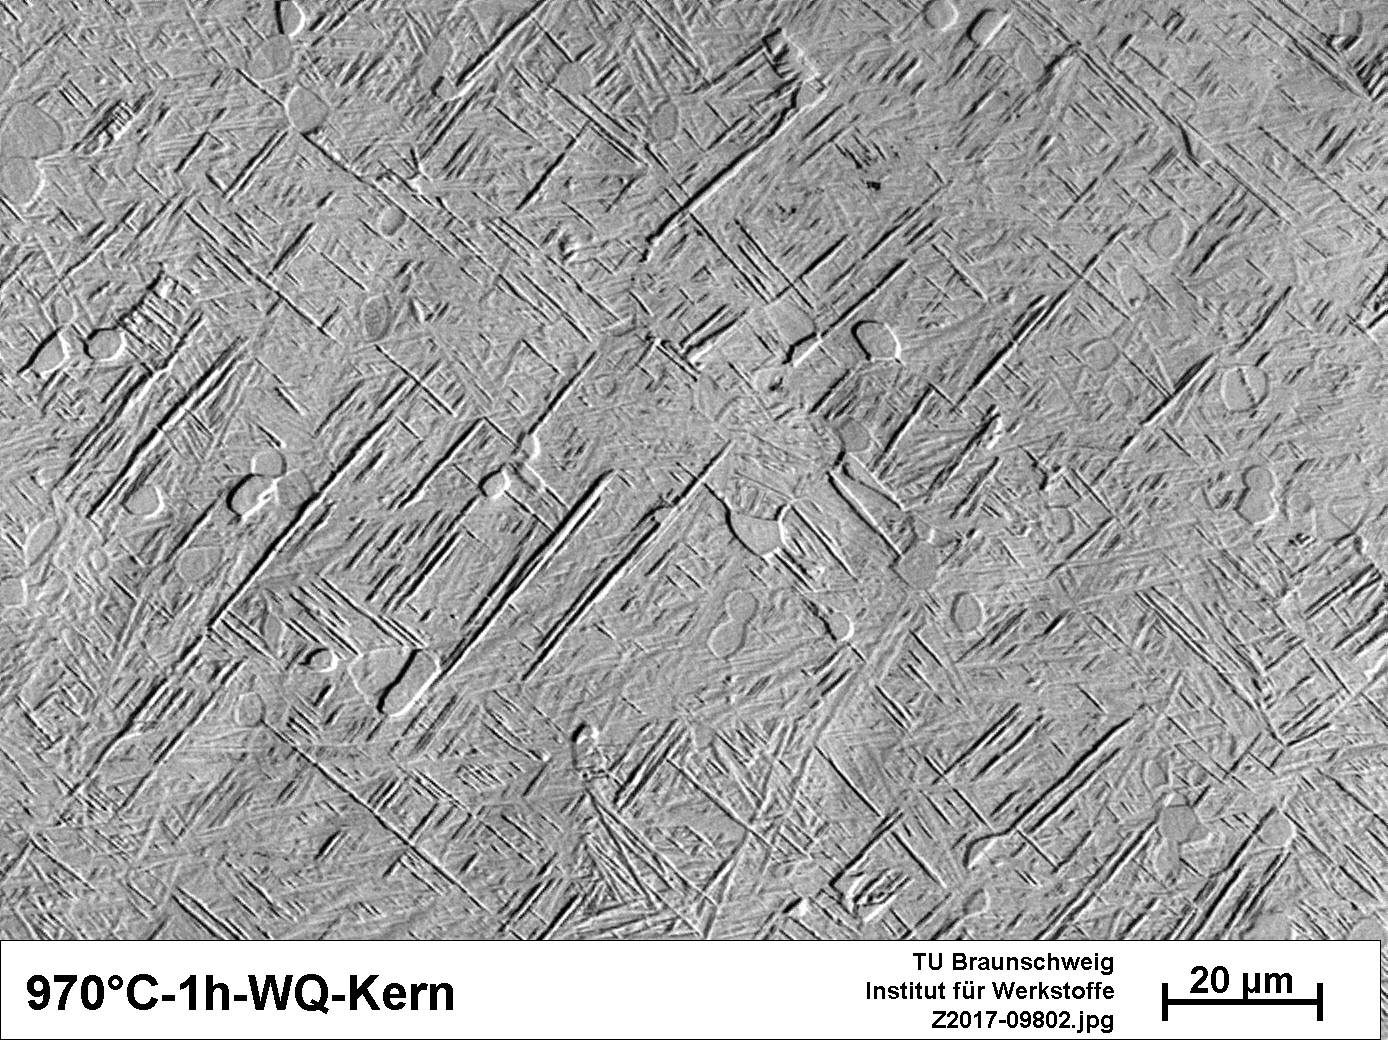
\includegraphics[width=0.33\textwidth]{Bilder/9701hwq.jpg}}
\subfigure[Gefüge bei einer Glühungstemperatur von 960°C]{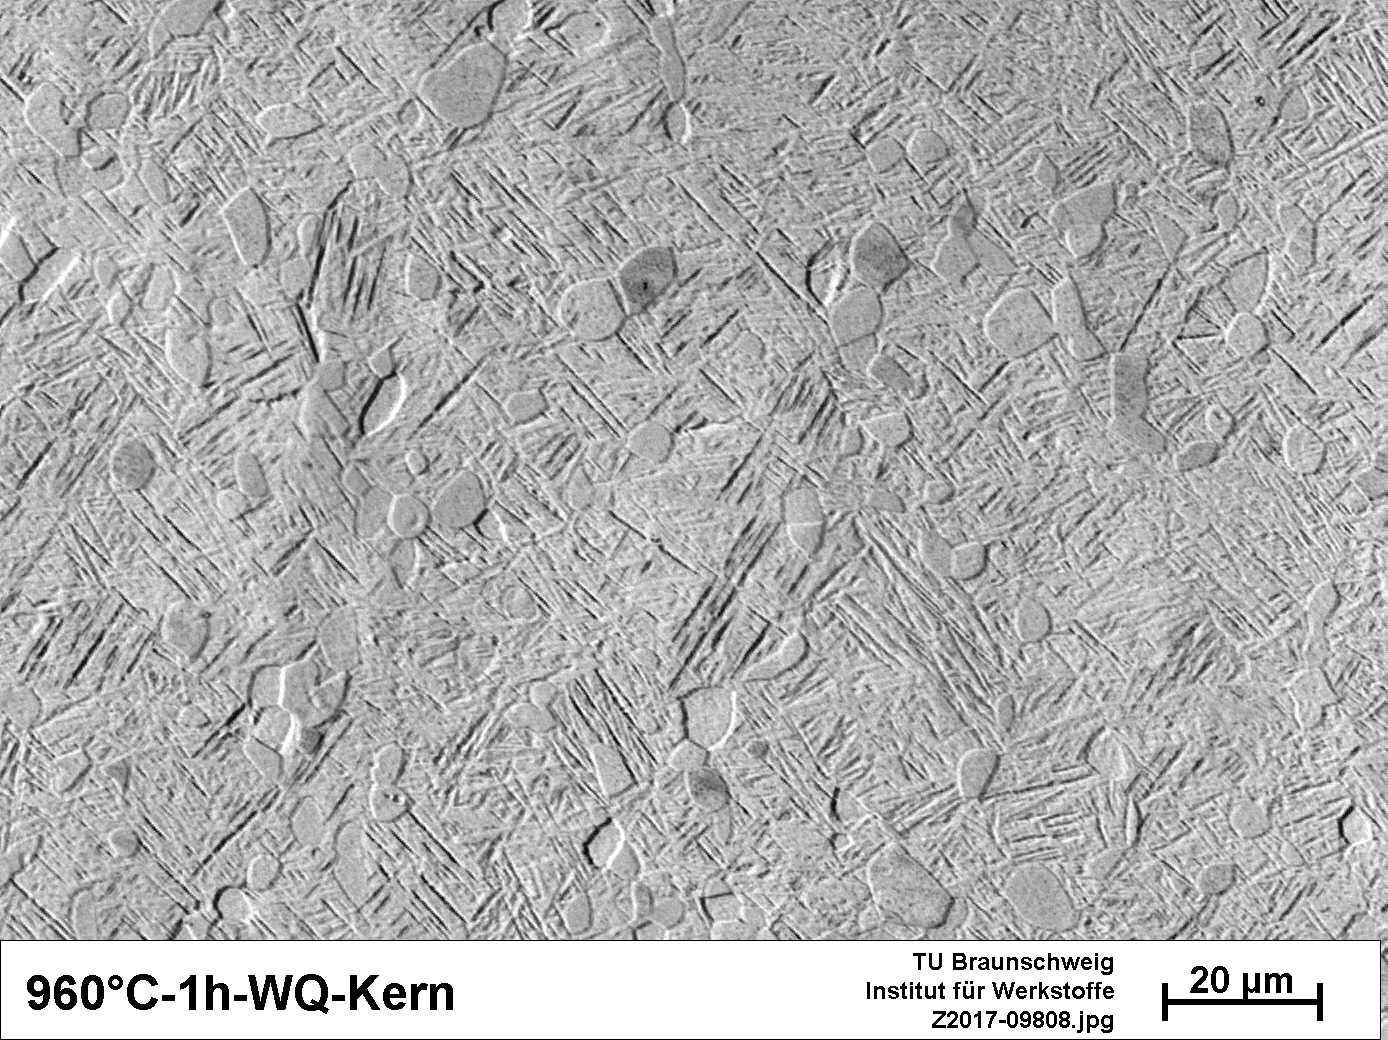
\includegraphics[width=0.33\textwidth]{Bilder/9601hwq.jpg}}
\subfigure[Gefüge bei einer Glühungstemperatur von 950°C]{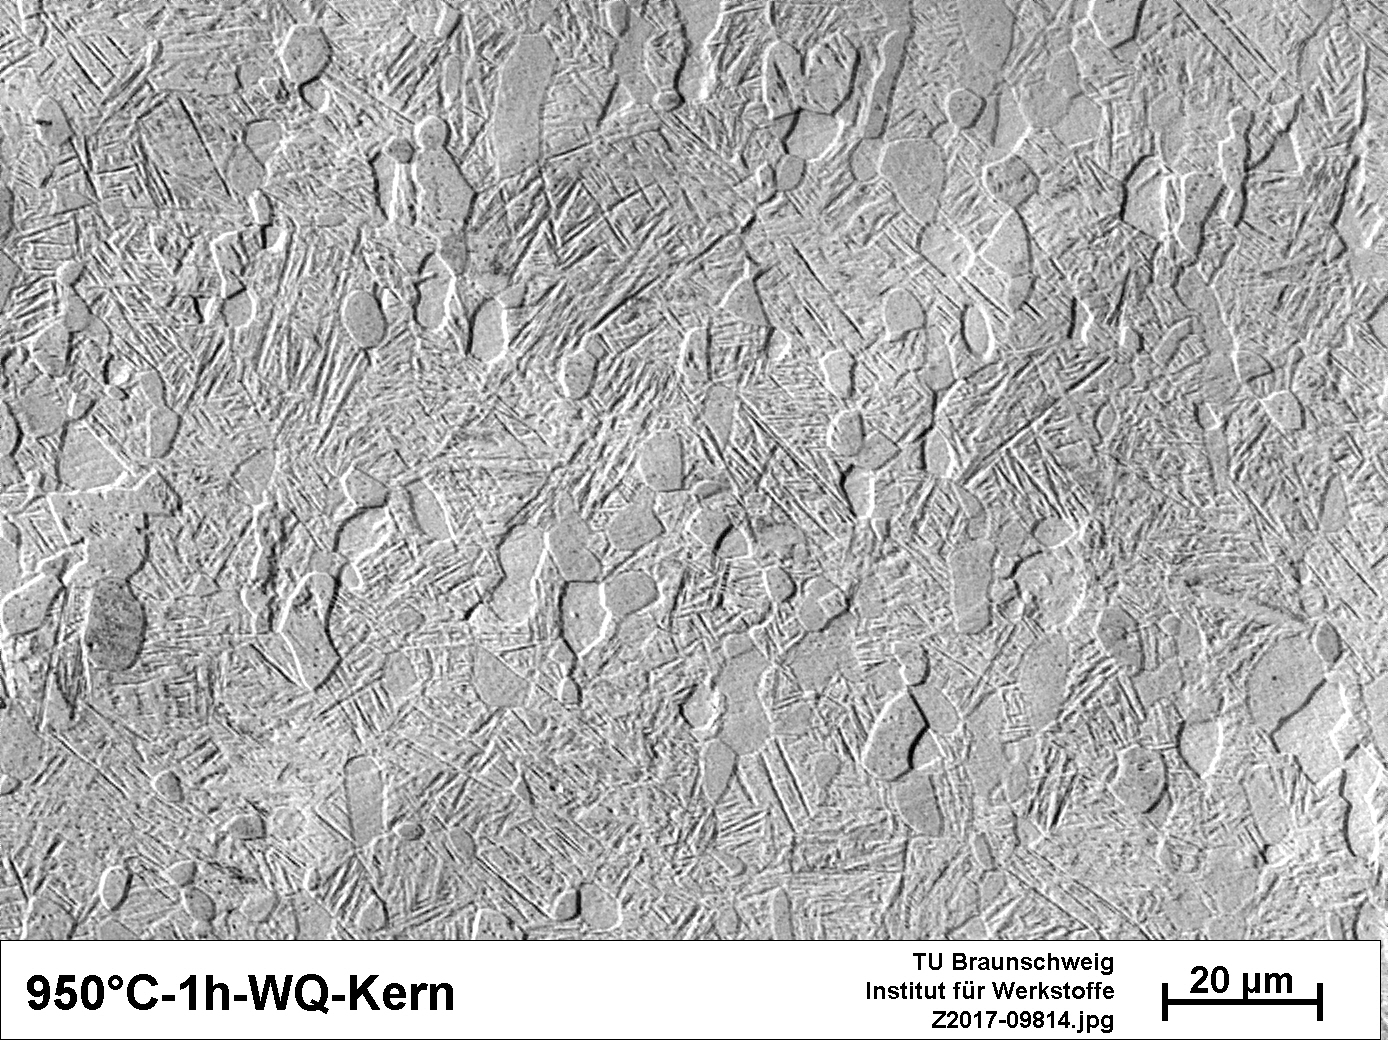
\includegraphics[width=0.33\textwidth]{Bilder/9501hwq.jpg}}
\caption{Gefüge unterschiedlicher Glühtemperaturen}
\label{Alle Glühen}
\end{figure}

Die genauen Phasenanteile wurden mittels Auszählverfahren (2.2.1) bestimmt. Die Ergebnisse zeigt Tabelle \ref{Tabelle Primäralphaanteil}.Bei einer Temperatur von 970°C ist der Alpha Anteil mit  6 \% sehr gering und mittels Lichtmikroskop nur noch schwer zu erkennen. Die 20 \% Alpha bei einer Glühtemperatur von 950°C hingegen sind noch deutlich zu erfassen.
\begin{table}
\begin{tabular}{c | c | c}
Wärmebehandlung & Mittelwert Primäralphaanteil \% & Standardabweichung \\
\hline
950°C 1h WQ	& 20 	&	1,57 \\
960°C 1h WQ	& 13 	&	1,68 \\
970°C 1h WQ	& 6  	&	1,82 \\
\end{tabular}
\caption{Primäralphaanteil in Abhängigkeit der Glühtemperatur}
\label{Tabelle Primäralphaanteil}
\end{table}

\subsection{Abhängigkeit der Härte vom Primäralphaanteil}
Die Härte der Proben wurde mittels der Vickers Härteprüfung bestimmt. Aus fünf Härtemessungen pro Probe wurde ein Mittelwert errechnet. Bei einer Prüfkraft von 10HV dringt der Prüfkörper in die Alpha Körner und den Martensit ein. Somit entsteht in gemitteltem Härtewert des Gefüges. Die Tabelle \ref{Härte in Abhängigkeit der Glühtemperatur} zeigt eindeutig, dass die Härte mit sinkendem Primär Alpha Anteil steigt. Bei einem Anteil von 20 \% liegt die Härte bei ca. 340 HV10. Sinkt der Anteil auf 6 \%, steigt die Härte auf einen Wert von ca. 360 HV10.

\begin{table}	%Härte in Abhängigkeit der Glühtemperatur
\begin{tabular}{c|c|c|c}
Wärmebehandlung	& Primär Alpha Anteil [\%] &	Mittelwert 
Härte in HV10 	& Standardabweichung \\
\hline
950°C 1h WQ	& 	20	&	343	&	6,68 \\
960°C 1h WQ	&	13	&	351	&	9,07 \\
970°C 1h WQ	&	6	&	357	&	8,95 \\

\end{tabular}
\caption{Härte in Abhängigkeit der Glühtemperatur}
\label{Härte in Abhängigkeit der Glühtemperatur}
\end{table}
\subsection{Bewertung der Ergebnisse}
Es besteht eine Proportionalität zwischen dem Primär Alpha Anteil und der Härte des Gefüges. Je geringer der Anteil Alpha Phase im Gefüge, desto höher ist die Härte. Der wachsende Anteil des Martensits bewirkt somit die Härtesteigerung. Mit diesem Ergebnis ist zu klären, ob ein vollmartensitisches Gefüge die Härte nochmals steigert. Dieses Gefüge wird im vollgendem behandelt.
Zudem ist die hohe Standardabweichung der Härtewerte auffällig (siehe Anhang Härte Protokolle). Die Härteeindrücke wurden längs durch die Schlifffläche gelegt. Die Härteprotokolle zeigen, dass der erste und der fünfte Messwert oft nach unten ausreißt. Diese Eindrücke liegen nahe der Randzone. Ein Härteabfall in der Randzone könnte mit dem entstandenen $\alpha$-Case \ref{alphacase} zusammen hängen.   

\begin{figure}
\centering
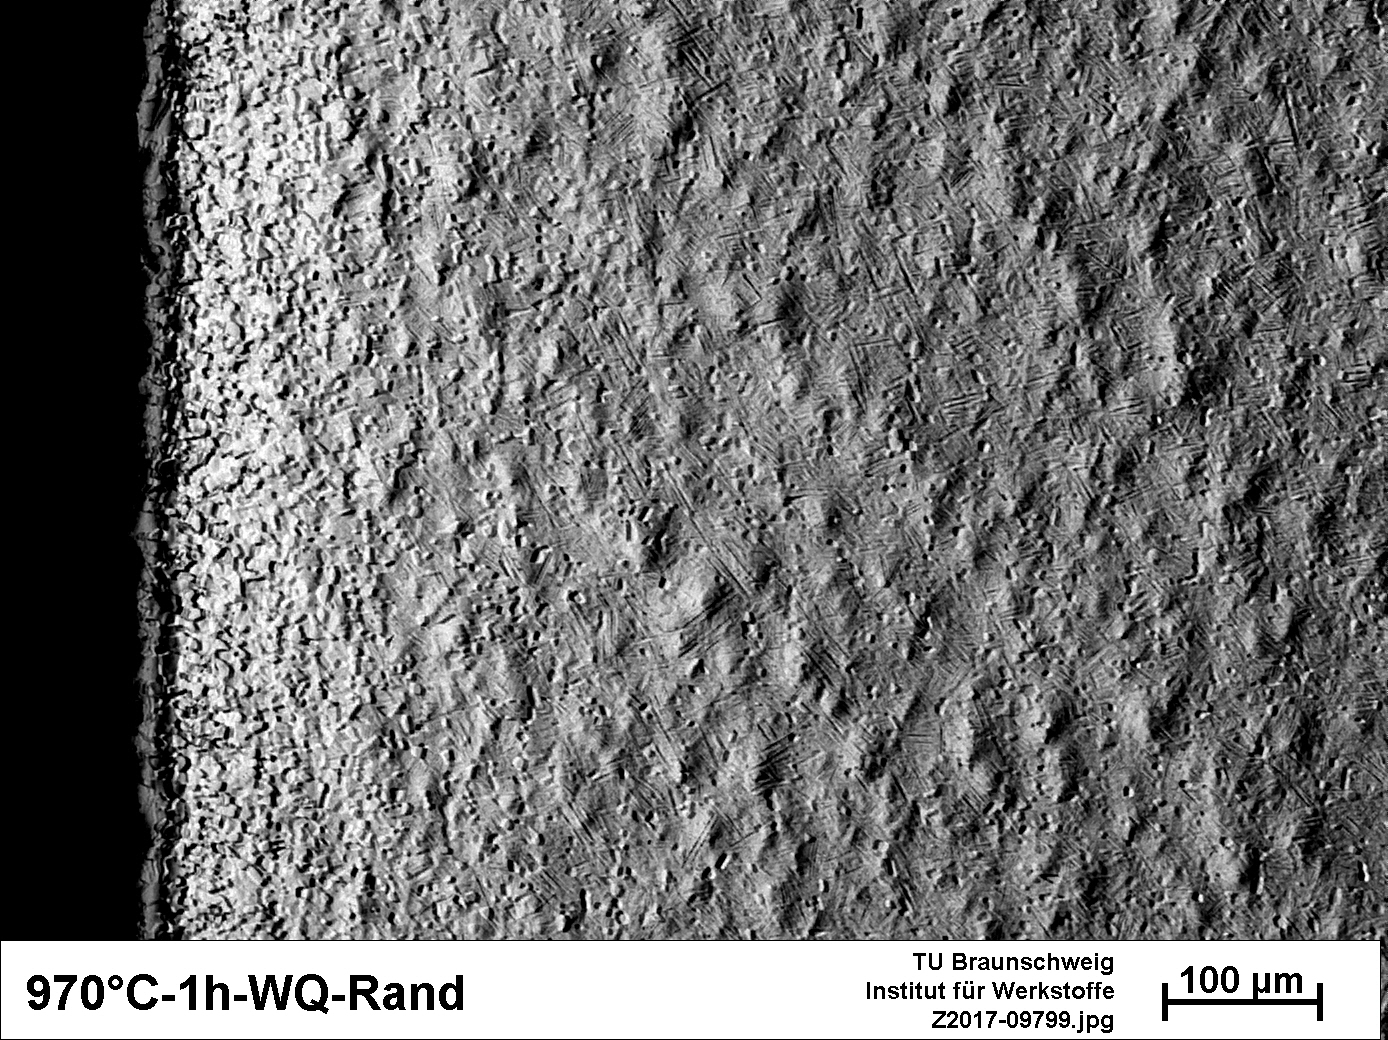
\includegraphics[width=0.5\textwidth]{Bilder/alphacase.jpg}
\caption{Alphacase}
\label{alphacase}
\end{figure}  




\section{Festigkeitssteigerung durch Auslagern des Vollmatensits}
\section{Festigkeitssteigerung durch Auslagern von Primäralpha und Martensit}\label{Primäralpha und martensit}
In zahlreichen vergleichbaren Untersuchungen wurde bereits eine Festigkeitssteigerung durch Auslagerung von $\alpha + \alpha'$-Gefügen festgestellt. Auf Basis dieser Untersuchungen und von Ergebnissen aus vorherigen Behandlungen werden die Parameter für diese Wärmebehandlung gewählt. Ziel dieser Behandlung ist, den metastabilen Martensit in sekundäre Alpha- und Beta-Phase zerfallen zu lassen. Es ergeben sich so größere Festigkeiten und bessere mechanische Eigenschaften \cite{Gilbert2004}. Es konkurrieren jedoch zwei Mechanismen bei einer Alterung des Martensits. Zum einen werden die Nadeln innerhalb des Martensits breiter, sodass eine Abnahme der Härte aufgrund geringerer Grenzflächendichte folgt. Der andere Mechanismus ist der Zerfall des Martensits in feine Alpha- und Betakörner die sich innerhalb des Gefüges bilden. Diese feinen Körner sorgen für eine Festigkeitssteigerung. Es ist also das Ziel, die Vergröberung des Gefüges zu minimieren, während der Zerfall maximiert werden soll. 
\subsection{1. Wärmebehandlung}
Wärmebehandlungen wie in \cite{Gilbert2004} und \cite{Chen2008} geben Beispiele für erfolgreiche Glüh- und Alterungsprozesse. Sie dienen als Hilfsmittel für die Parameterwahl bei dieser Wärmebehandlung. Bei den Bespielen werden Glühtemperaturen von 950°C bis 970°C verwendet, sodass ein zweiphasiges Gefüge mit unterschiedlichen Primäralpha-Gehalten entsteht. Um neben dem Primäralpha ein Martensit zu erzeugen, wird in Wasser abgeschreckt. Für einen vollständigen Abschluss der Diffusionsvorgänge wird wie in der Wärmebehandlung aus Kapitel \ref{Festigkeitssteigerung durch Martensitbildung} eine Haltezeit von einer Stunde als ausreichend eingestuft.

Wie vorherige Wärmebehandlungen zeigen, wirkt sich ein geringer Primäralpha Anteil positiv auf die Härte beziehungsweise Festigkeit aus. Für den Zerfall des Martensits ist jedoch die Konzentration an Beta stabilisierender Elemente in der Martensitphase entscheidend. Diese liegt wie in den EDX-Ergebnissen aus Kapitel \ref{Festigkeitssteigerung durch Martensitbildung} niedriger, je kleiner der Primäralpha-Anteil ist. Demnach könnten Proben mit einem niedrigeren Primäralpha-Anteil durch eine Alterung geringere Festigkeiten aufweisen als Proben mit höheren Primäralpha-Anteilen.

Für die Alterung, mit anschließender Luftkühlung, wurde in den Behandlungen aus den Quellen eine Temperatur von 490°C bis 595°C und eine Haltezeit von 1 bis 8 Stunden angegeben. Da diese Spanne sehr groß ist und eine aussagekräftige Beurteilung der Ergebnisse für den gesamten Bereich unverhältnismäßig aufwendig sein würde, wurden zwei Temperaturen festgelegt und über die Haltezeit variiert. So werden in einem ersten Schritt die Auswirkungen des Primäralpha-Anteils analysiert. Es wurden Wasser abgeschreckte Proben bei einer Glühtemperatur von 970°C und 950°C jeweils zwei und acht Stunden bei 520°C gealtert. Es werden also vier Proben verwendet, die ein vergleichbares Ergebnis liefern sollen. So kann eine Auswirkung der unterschiedlichen Primäralpha-Anteile gleichzeitig mit der Auswirkung der Haltedauer beobachtet werden und Rückschlüsse auf die entstehenden Eigenschaften getroffen werden.
\subsection{Ergebnisse 1. Wärmebehandlung}
\subsubsection{970°C Auslagerung}
Auf den Gefügebildern mit dem Lichtbildmikroskop aus Abbildung \ref{970 alterung} sind kaum Unterscheide zu dem Ausgangsgefüge aus Abbildung \ref{Gefüge ohne Alterung}(a) zu sehen. Die Primäralpha Phase ist unabhängig von der Auslagerungszeit in ihrer Ausdehnung konstant geblieben. Der Martensit hat sich unter dem Lichtmikroskop nicht verändert. Falls die Martensit-Phase sich in ihrer Struktur verändert hat, ist dies nur unter einem REM zu sehen. Ein Zerfall würde sich nur in kleinen Teilchen äußern, die in dieser Vergrößerung nicht zu sehen sind. 


Die REM-Aufnahme aus Abbildung \ref{REM 970C und 950C}(a) zeigt das Gefüge von einem Abschrecken von 970°C. Wird diese Aufnahme mit denen nach dem Altern aus Abbildung \ref{REM 970C auslagerung} verglichen, fallen Unterschiede auf. Der gealterte Martensit hat eine ungleichmäßigere, ''körnigere''  Struktur als der nicht ausgelagerte. Diese Struktur ist bei der Probe mit längerer Haltezeit noch gröber. 
\begin{figure}
\subfigure[Glühen bei 970°C]{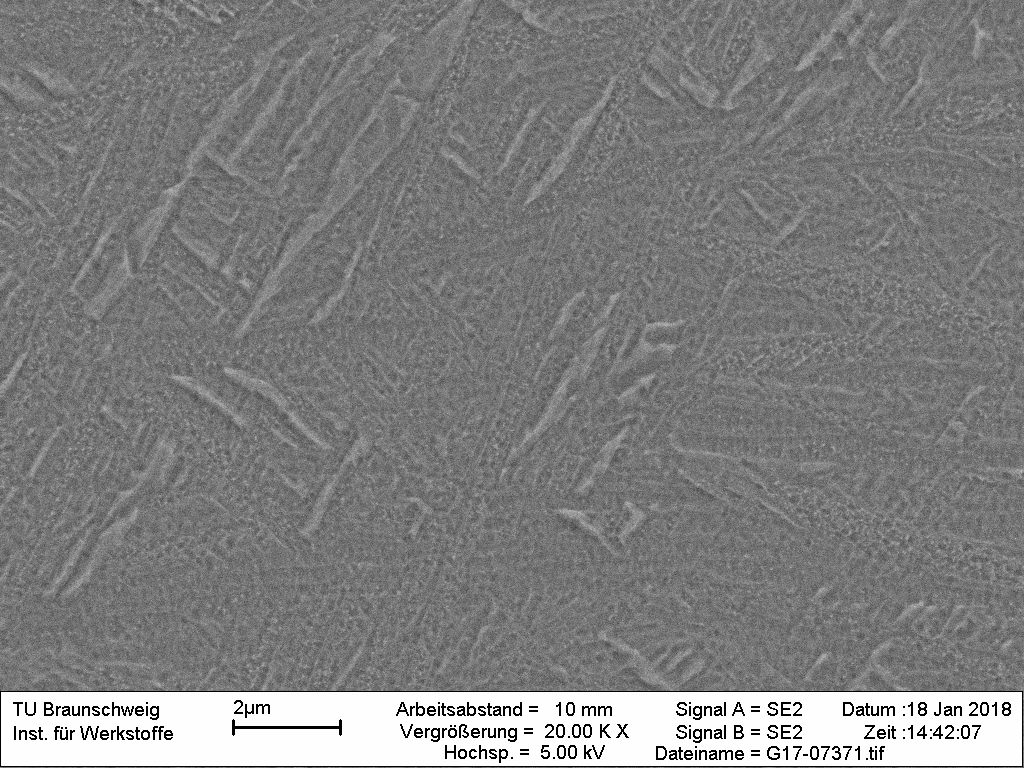
\includegraphics[width=0.5\textwidth]{Bilder/REM970C1hWQ.png}}
\subfigure[Glühen bei 950°C]{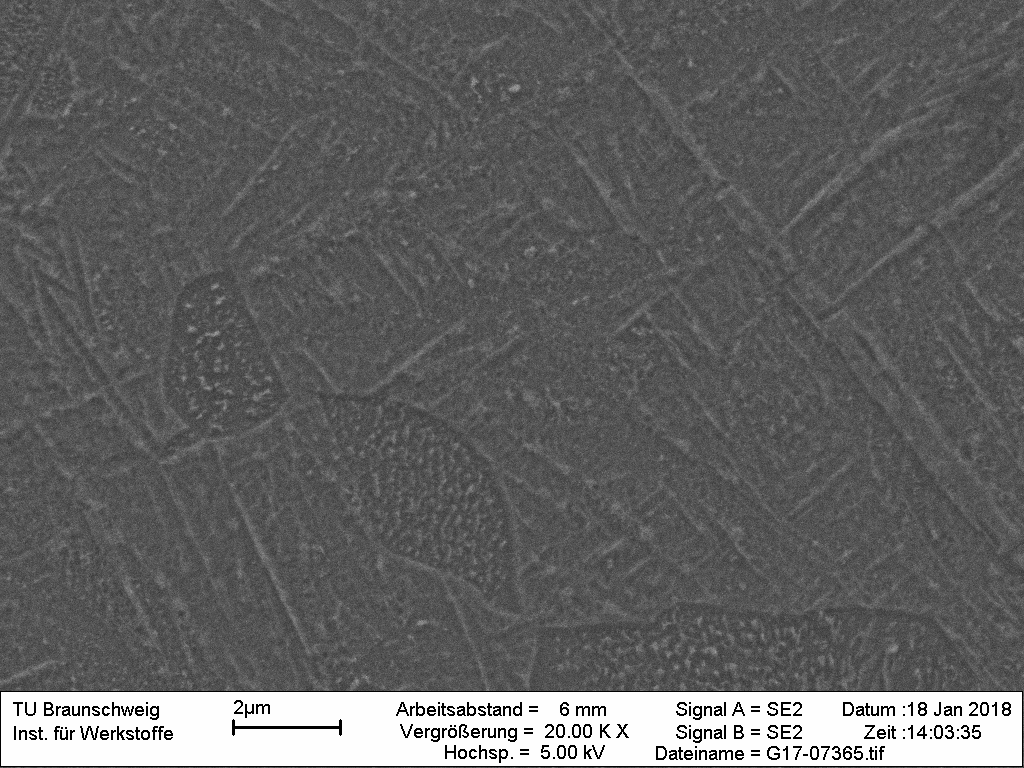
\includegraphics[width=0.5\textwidth]{Bilder/REM950C1hWQ.png}}
\caption{REM Bilder abschrecken von 950°C und 970°C}
\label{REM 970C und 950C}
\end{figure}


\begin{figure}
\subfigure[Zwei Stunden Alterung]{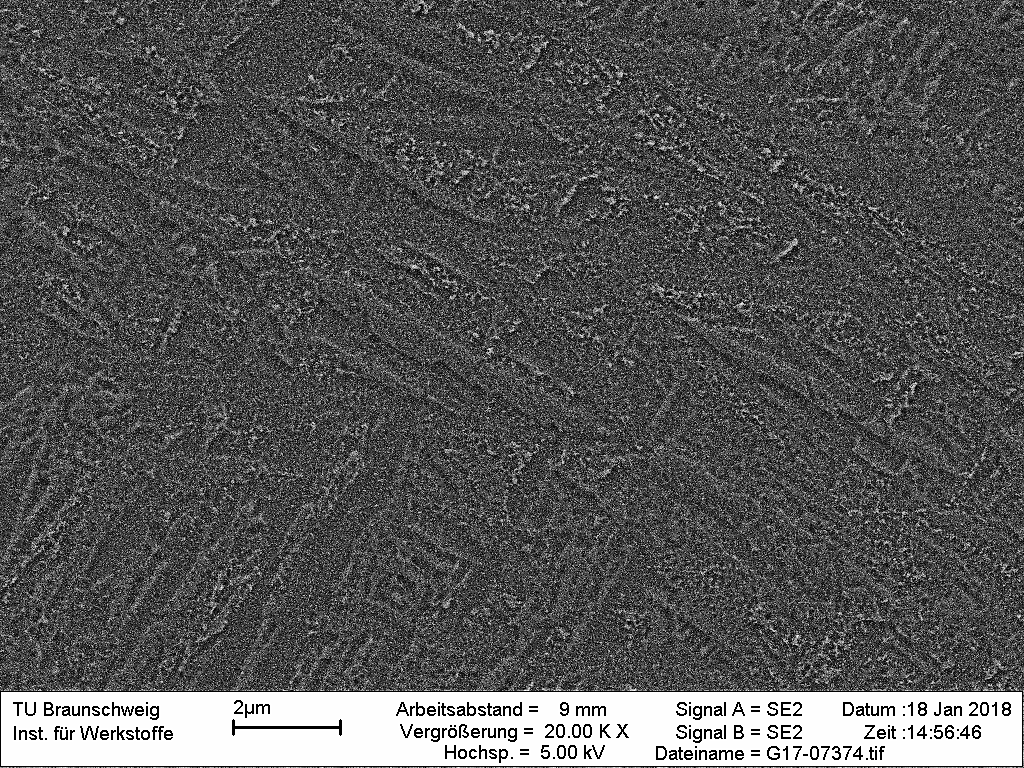
\includegraphics[width=0.5\textwidth]{Bilder/REM970C1hWQ520C2hAC.png}}
\subfigure[acht Stunden Alterung]{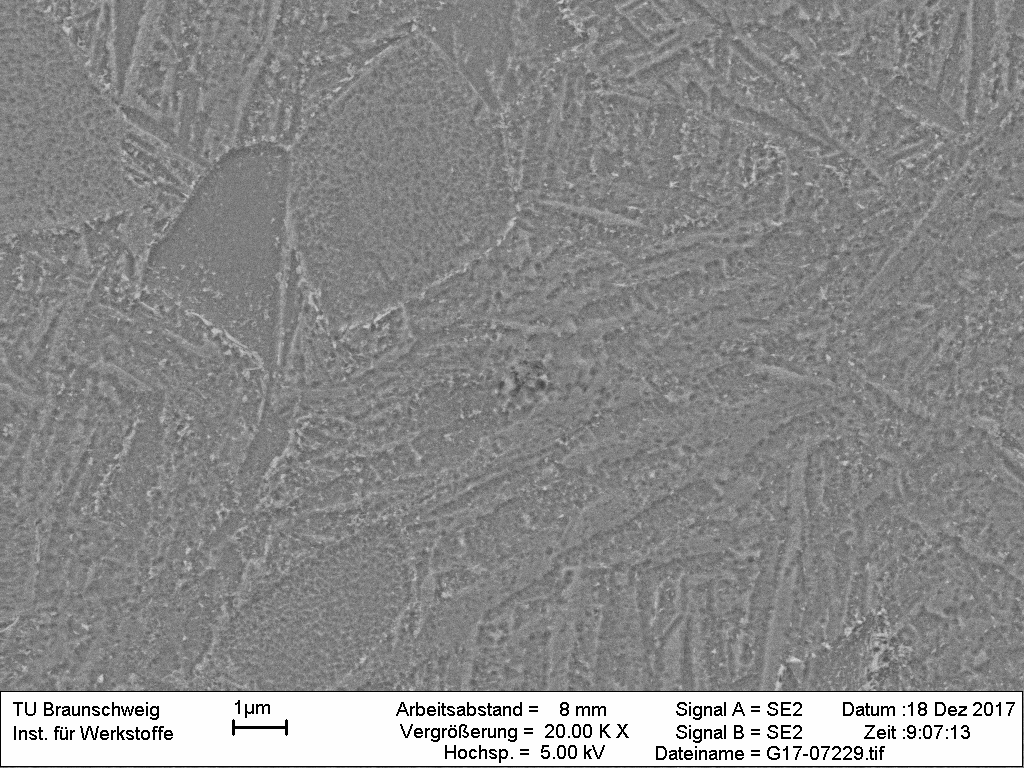
\includegraphics[width=0.5\textwidth]{Bilder/REM970C1hWQ520C8hAC.png}}
\caption{Gefüge der gealterten Proben Glühen bei 970°C}
\label{REM 970C auslagerung}
\end{figure}


Durch eine Härteprüfung lässt sich die Auswirkung der Alterung analysieren. Dabei wird das in Kapitel zwei beschriebene Verfahren angewendet. Für die Behandlungsreihe mit 970°C ergeben sich die Ergebnisse aus Tabelle \ref{heartepruefung970 inkl auslagern}. Ein Vergleich mit den Härtewerten der nicht ausgelagerten Probe aus Tabelle \ref{Hearte ohne Behandlung} zeigt keine Härtesteigerung. 
\subsubsection{950°C Auslagerung}
Wie auch schon bei den Proben bei 970°C sind unter dem Lichtmikroskop keine Unterschiede zwischen den ausgelagerten Proben und der unbehandelten Probe zu erkennen. Für eine genauere Analyse muss also ein REM herangezogen werden.

Die Bilder des REM aus Abbildung \ref{REM 950 2 und 8} zeigen das resultierende Gefüge nach den jeweiligen Haltezeiten. Es sind ähnliche Ergebnisse wie bei der Alterung der Glühtemperatur von 970°C zu erkennen. Der Martensit hat seine charakteristische Struktur verloren. Die nach dem Abschrecken entstandenen Nadeln sind nur noch in keinen Mengen zu sehen. Ein Großteil ist in vielen Stellen unterbrochen und gröber geworden. Es ist schwierig, einen Unterschied des Gefüges aufgrund der Haltezeit zu erkennen. Die Struktur ist mit der Zeit noch gröber geworden und die Anzahl der Unterbrechungen ist größer geworden.
\begin{figure}
\subfigure[2 Stunden Haltezeit]{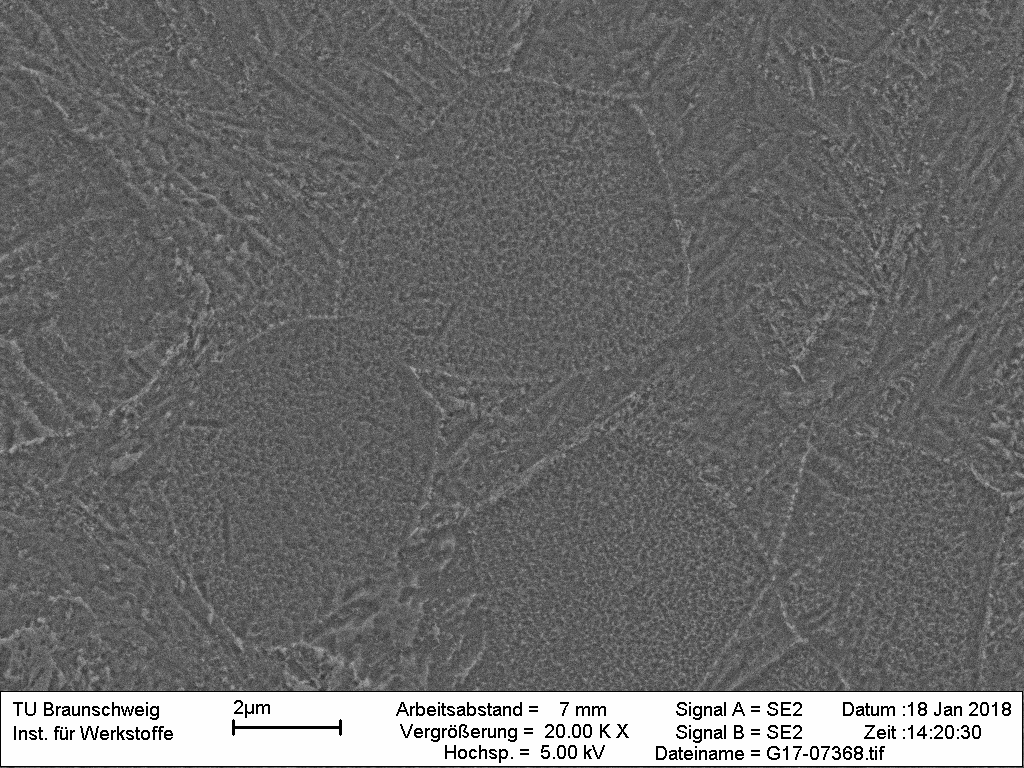
\includegraphics[width=0.5\textwidth]{Bilder/REM9501hWQ520C2hAC.png}}
\subfigure[8 Stunden Haltezeit]{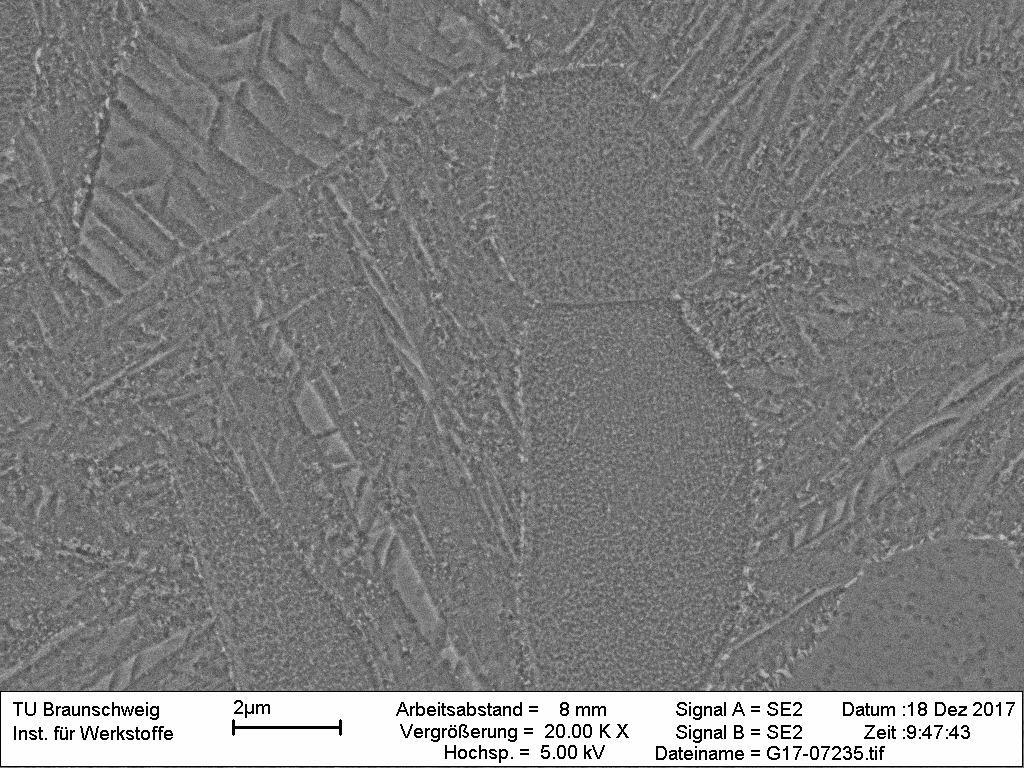
\includegraphics[width=0.5\textwidth]{Bilder/REM950C1hWQ520C8hAC.png}}
\label{REM 950 2 und 8}
\caption{Auslagerung der Glühtemperatur 950°C bei 2 und 8 Stunden}
\end{figure}

Bei den Proben, die mit 950°C geglüht und zwei beziehungsweise acht Stunden bei 520°C ausgelagert wurden, zeigt sich ein anderes Ergebnis der Härteprüfung als bei den Proben bei einer Glühtemperatur von 970°C. Wenn die Härtewerte nach der Alterung mit denen vorher verglichen werden, ist eine Härtesteigerung erkennbar. Die Werte aus der Tabelle \ref{950alterung} sind im Schnitt 10 HV10 höher als das Material vor der Behandlung. Die verwendeten Haltezeiten weisen keinen Unterschied hinsichtlich der Härte auf. Sie liegen für beide Zeiten bei circa 360 HV 10.
\begin{table}[t]	%Härtewerte ohne Auslagerung
\begin{tabular}{c|c}
\multicolumn{2}{c}{970°C 1h WQ} \\
\hline 
Abstand in mm	& Härte in HV10 \\
0.02	& 342\\
2.92	& 362\\
5.80	& 363\\
8.69	& 363 \\
11.58	& 355\\
\hline
Mittelwert	& 357 \\
Max	& 363 \\
Min.	& 342 \\
Std.-abw. &	8.95 \\

\end{tabular}
\begin{tabular}{c|c}
\multicolumn{2}{c}{950°C 1h WQ} \\
\hline 	
Abstand in mm	& 	Härte in HV10 \\
-0.01	&	337 \\
3.17	&	347 \\
6.32	&	349 \\
9.48	&	348 \\ 
12.62	&	336 \\
\hline
Mittelwert &	343 \\
Max	&	349 \\
Min.	&	336 \\
Std.-abw.	&	6.68 \\

\end{tabular}
\caption{Härtewerte ohne Auslagerung}
\label{Hearte ohne Behandlung}
\end{table}
\begin{table}[t] 	%Härteprüfung 970°C Glühen und Auslagern
\begin{tabular}{c | c}
\multicolumn{2}{c}{2h Auslagern} \\
\cline{1-2}
Abstand in mm & Härte in HV10 \\
0.03 & 357 \\
3.16 & 358 \\
6.29 & 360 \\
9.43 & 354 \\
12.56 & 359 \\
\hline
Mittelwert & 358 \\
Max & 360 \\
Min & 354 \\
Std.-abw. & 2.58 \\
\end{tabular}
\begin{tabular}{c | c}
\multicolumn{2}{c}{8h Auslagern} \\
\cline{1-2}
Abstand in mm & Härte in HV10 \\
0.07	&		353 \\
2.91	&		352 \\
5.79	&		352\\
8.67	& 		355\\
11.54	& 		357\\
\hline
Mittelwert &	354\\
Max	& 			357\\
Min. &			352	\\	
Std.-abw.	&	2.40\\

\end{tabular}
\caption{Härteprüfung 970°C Glühen und Auslagern}
\label{heartepruefung970 inkl auslagern}
\end{table}
\begin{table}[t] 	%950 Alterung
\begin{tabular}{c|c}
\multicolumn{2}{c}{2h Auslagern} \\
\hline
Abstand in mm	& Härte in HV10 \\
0.01	&	352 \\
2.98	&	356 \\
5.94	&	356 \\
8.90	&	355 \\
11.86	&	358 \\
\hline
Mittelwert	&	355 \\
Max	&	358 \\
Min.	&	352 \\
Std.-abw.	&	2.43 \\

\end{tabular}
\begin{tabular}{c|c}
\multicolumn{2}{c}{8h Auslagern} \\
\hline
Abstand in mm	&	Härte in HV10 \\
0.02	&	357 \\
3.22	&	355 \\
6.42	&	358 \\
9.62	&	357 \\
12.82	&	354 \\
\hline
Mittelwert	&	356 \\
Max	&	358 \\
Min.	&	354 \\
Std.-abw.	&	1.83 \\

\end{tabular}
\caption{Härteprüfung 950°C Glühen und Auslagern}
\label{950alterung}
\end{table}
\begin{figure} 		%Gefüge Ohne Alterung
	\subfigure[Gefüge bei einer Glühungstemperatur von 970°C ohne Alterung]{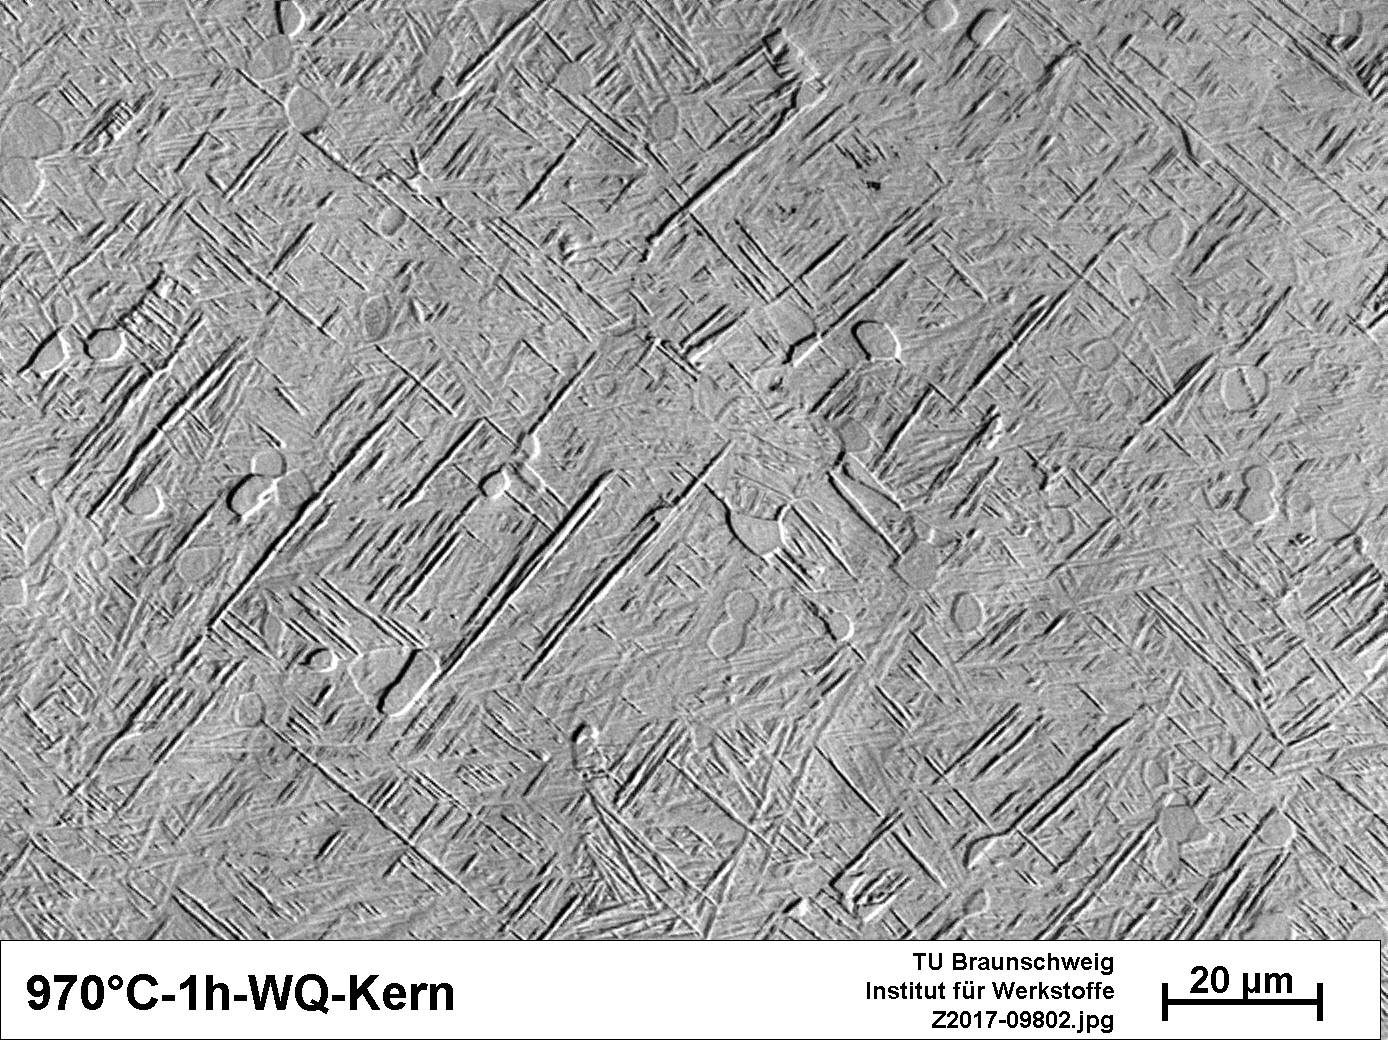
\includegraphics[width=0.49\textwidth]{Bilder/9701hwq.jpg}} 
    \subfigure[Gefüge bei einer Glühungstemperatur von 950°C ohne Alterung]{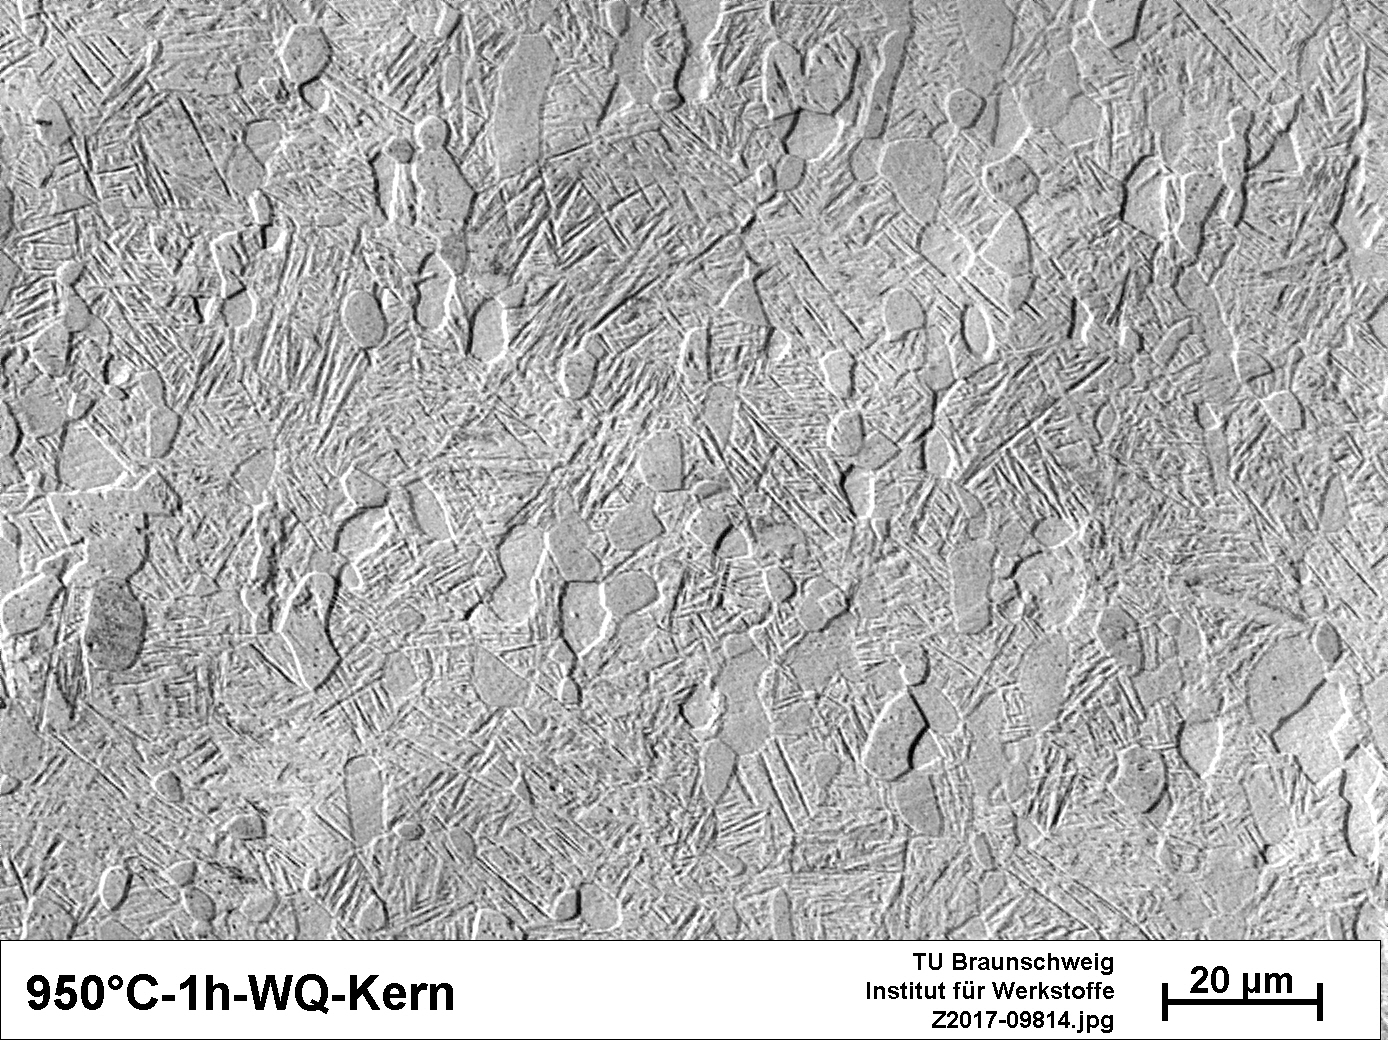
\includegraphics[width=0.49\textwidth]{Bilder/9501hwq.jpg}} 
	\caption{Gefüge ohne Auslagern}
	\label{Gefüge ohne Alterung}
\end{figure}
\begin{figure} 		%970°C und alterung
	\subfigure[Gefüge bei einer Glühungstemperatur von 970°C mit Auslagerung bei 520°C für 2h]{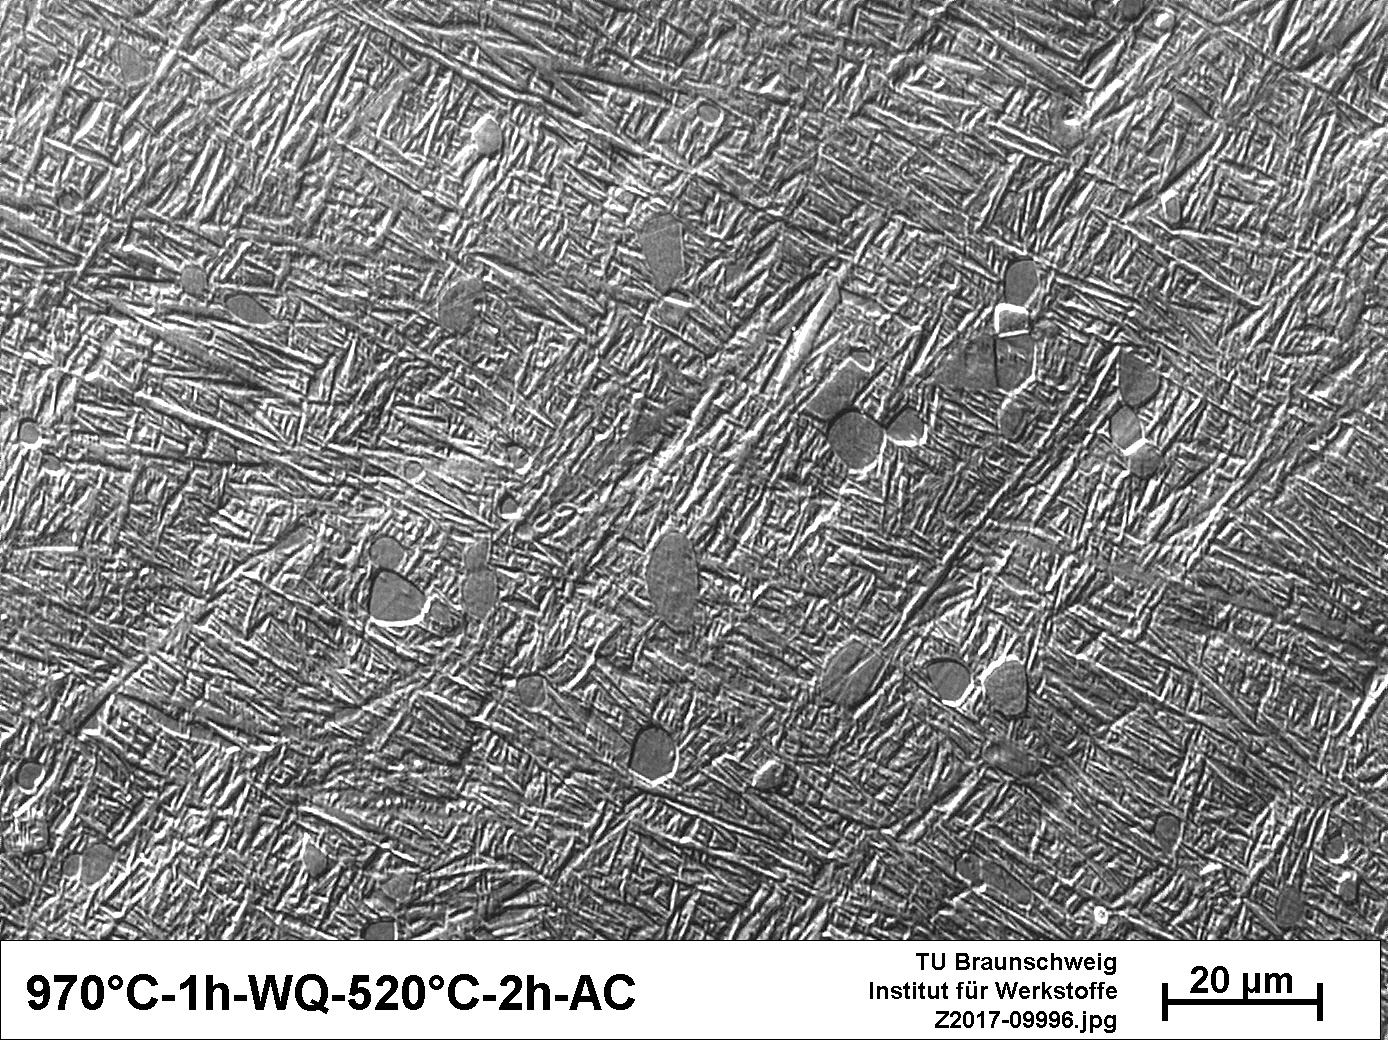
\includegraphics[width=0.49\textwidth]{Bilder/9701hwq5202hac.jpg}} 
    \subfigure[Gefüge bei einer Glühungstemperatur von 970°C mit Auslagerung bei 520°C für 8h]{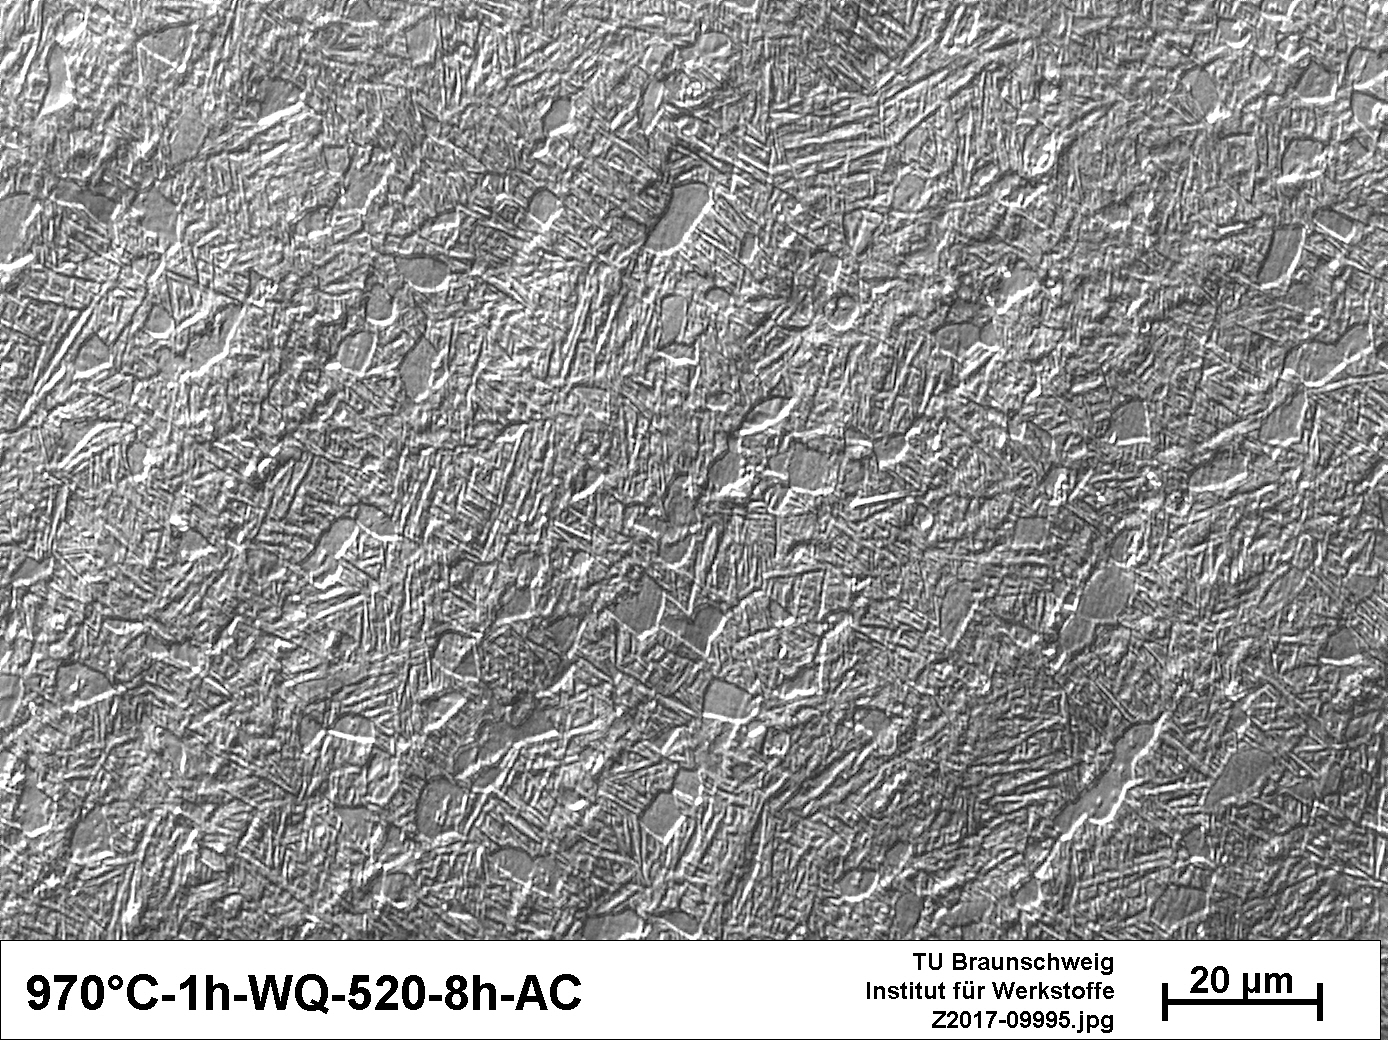
\includegraphics[width=0.49\textwidth]{Bilder/9701hwq5208hac.jpg}} 
    \caption{Gefüge mit einer Glühtemperatur von 970°C und unterschiedlichen Alterungszeiten}
    \label{970 alterung}
\end{figure}



\subsection{2. Wärmebehandlung}
Aus den Ergebnissen der ersten Wärmebehandlung lässt sich schließen, dass eine längere Haltezeit, innerhalb einer Auslagerung ausgehend von einer Glühtemperatur von 970°C, keine Festigkeitssteigerung hervorruft. Die Alterung der geringeren Glühtemperatur zeigt bereits eine Härtesteigerung von circa 3\%. Eine Zunahme der Härte bei längerer Haltezeit ist somit für die Proben mit einer Glühtemperatur von 970°C unwahrscheinlich. 

Da die Haltezeiten keinen Unterschied hinsichtlich der Härtesteigerung aufweisen, wird eine verlängerte Haltezeit angewendet. Es kann sein, dass der Zerfall des Martensits noch weiter fortschreitet, da während den verwendeten Haltezeiten die Diffusionsvorgänge nicht abgeschlossen werden konnten. Um dies zu prüfen und festzustellen, ob eine noch längere Haltezeit eine größere Härte steigernde Wirkung hervorruft, werden die Haltezeiten auf 16 und 24 Stunden angepasst. So lässt sich zeigen, ob der Zerfall des Martensits noch positiv hinsichtlich der Festigkeit statt finden kann. 



\begin{figure} %950°C und alterung
	\subfigure[Gefüge bei einer Glühungstemperatur von 950°C mit Auslagerung bei 520°C für 2h]		{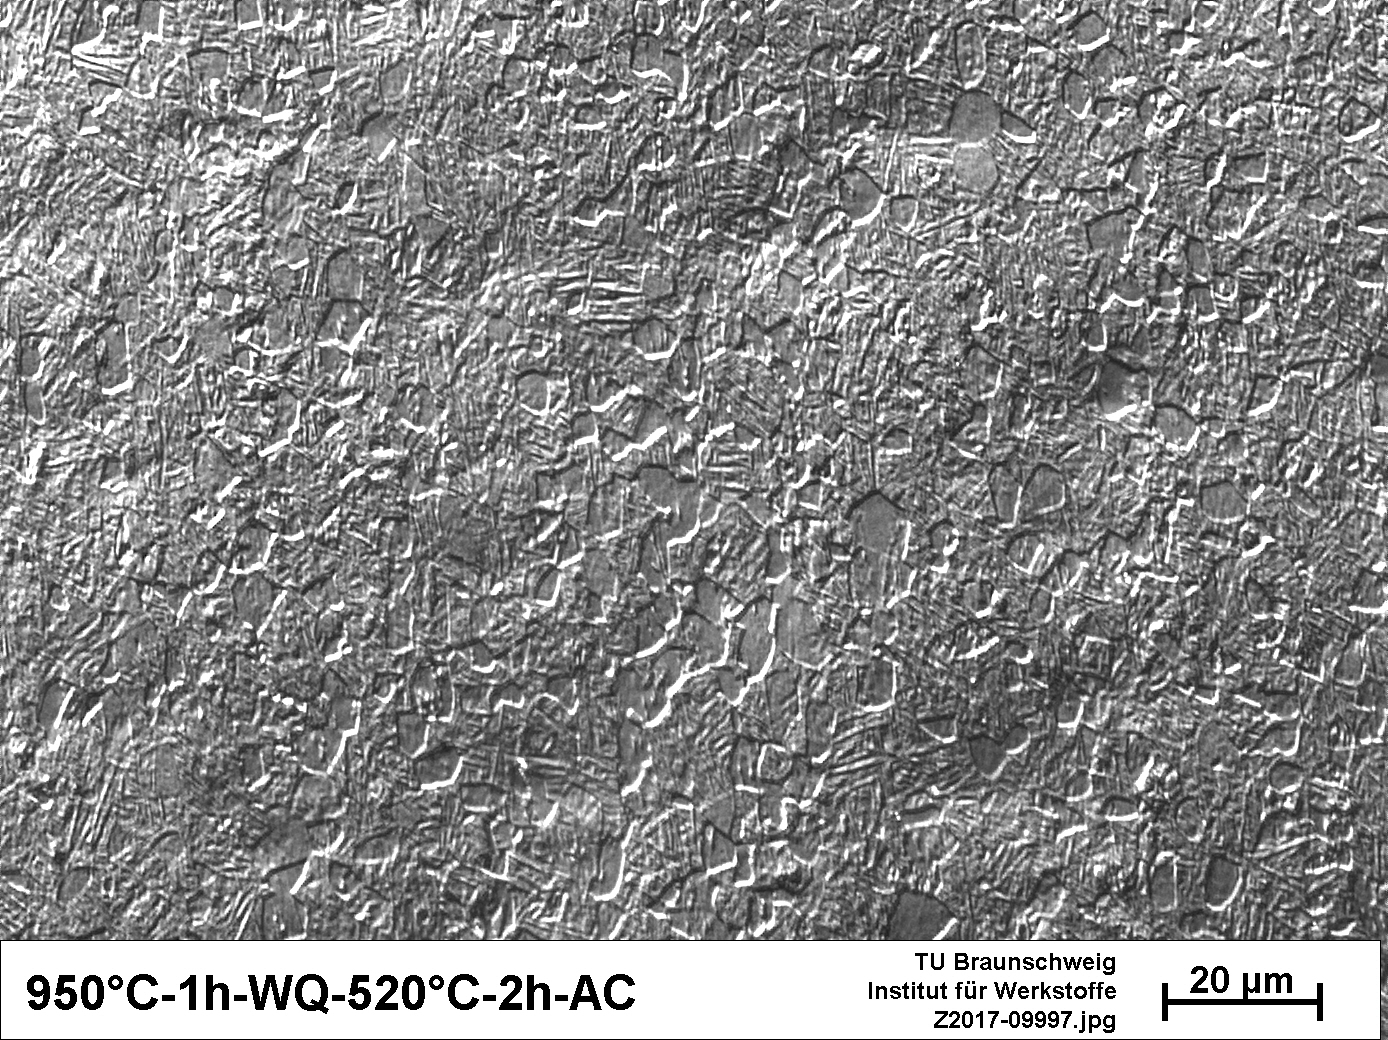
\includegraphics[width=0.49\textwidth]{Bilder/9501hwq5202hac.jpg}} 
    \subfigure[Gefüge bei einer Glühungstemperatur von 950°C mit Auslagerung bei 520°C für 8h]{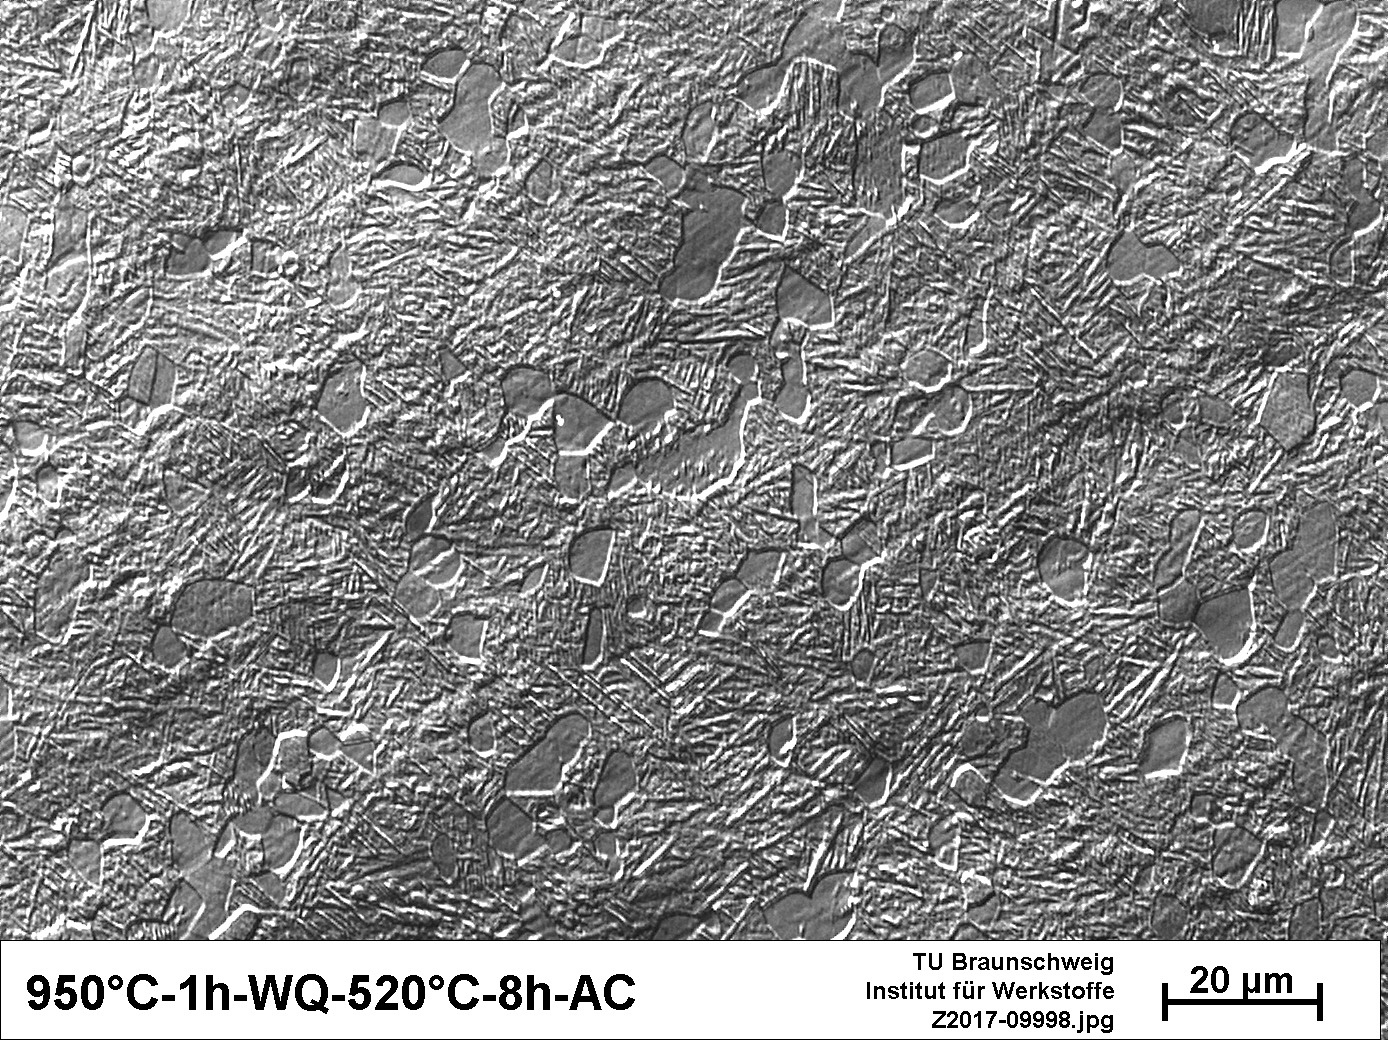
\includegraphics[width=0.49\textwidth]{Bilder/9501hwq5208hac.jpg}} 
    \caption{Gefüge mit einer Glühtemperatur von 950°C und unterschiedlichen Alterungszeiten}
    \label{Glühung950+alterung}
\end{figure}
\subsection{Ergebnisse 2. Wärmebehandlung}
Aus den Gefügebildern mit dem Lichtmikroskop aus Abbildung \ref{950 lange auslagerung} ist kein wesentlicher Unterschied erkennbar. Im Verhältnis zu der Probe, die nur zwei Stunden ausgelagert wurde, kann man eine leichte Verbreiterung der Nadeln erkennen. Jedoch ist eine mögliche Bildung von Alpha- und Beta-Phase unter dieser Auflösung nicht erkennbar. Dazu muss wie zuvor ein REM herangezogen werden.

Die Aufnahme aus Abbildung \ref{REM 950C 24h} zeigt eine REM-Aufnahme von dem 24 Stunden lang gealterten Gefüge. Das Martensit ist fast nicht mehr zu erkennen. Die ehemaligen Nadeln sind an vielen Stellen unterbrochen und als solche nicht mehr zu erkennen. Um das Alpha-Korn hat sich ein ausgeprägter Rand gebildet. Die für kürze Haltezeit beschriebene Vergröberung ist mit der Zeit noch einmal größer geworden.

Die Härtewerte zeigen, dass aus einer längeren Haltezeit eine höhere Härte resultiert. Im Vergleich zu der Haltezeit von zwei Stunden zeigen die Ergebnisse aus Tabelle \ref{950 16 24} für eine Haltezeit von 24 Stunden eine nochmalige Härtesteigerung von 10 HV10. Die Härte nimmt also für längere Haltezeiten stetig zu. 



\begin{figure}
\subfigure[Gefüge bei einer Glühungstemperatur von 950°C und 16 Stunden Alterung]{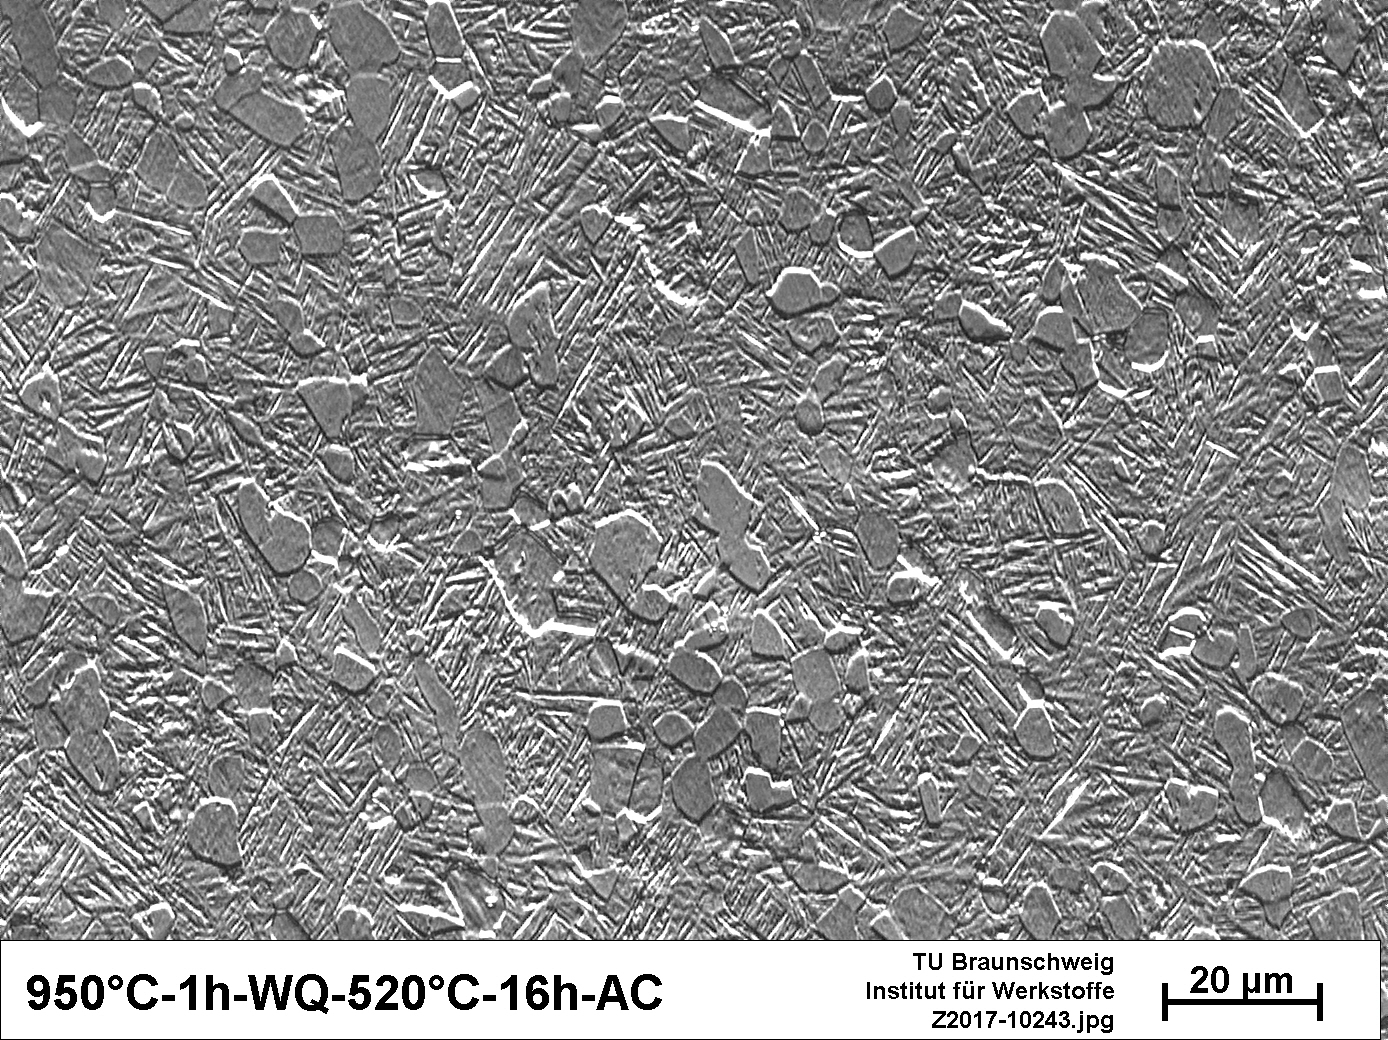
\includegraphics[width=0.49\textwidth]{Bilder/9501hwq52016hac.jpg}} 
    \subfigure[Gefüge bei einer Glühungstemperatur von 950°C und 24 Stunden Alterung]{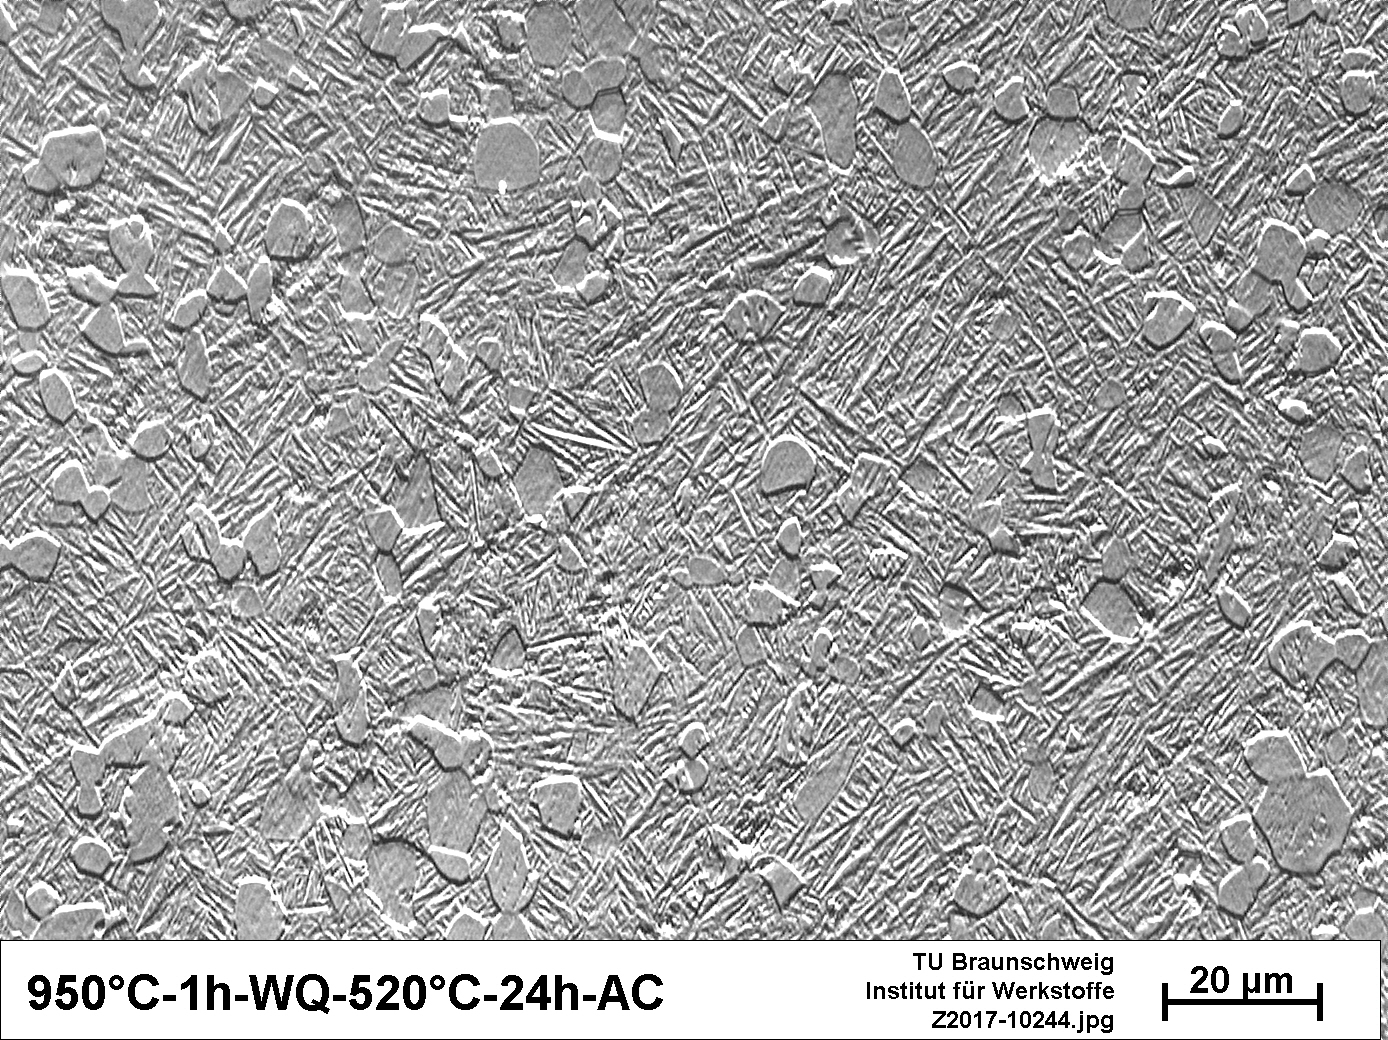
\includegraphics[width=0.49\textwidth]{Bilder/9501hwq52024hac.jpg}} 
	\caption{Gefüge bei 950°C bei 16h und 24h Auslagerung}
	\label{950 lange auslagerung}
\end{figure}

\begin{table}
\begin{tabular}{c|c}
\multicolumn{2}{c}{16h Auslagern} \\
\hline
Abstand in mm &	Härte in HV10 \\
0.02	&	359 \\
3.16	&	358 \\
6.31	&	362 \\
9.46	&	357 \\
12.60	&	360 \\
\hline
Mittelwert	&	359 \\
Max	&	362 \\
Min.	&	357 \\
Std.-abw.	&	1.79 \\
\end{tabular}
\begin{tabular}{c|c}
\multicolumn{2}{c}{24h Auslagern} \\
\hline
Abstand in mm	&	Härte in HV10 \\

0.02	&	362 \\
3.29	&	363 \\
6.55	&	363 \\
9.81	&	364 \\ 
13.07	&	363 \\
\hline
Mittelwert	&	363 \\
Max	&	364 \\
Min.	&	362 \\
Std.-abw.	&	0.803 \\
\end{tabular}
\caption{Härtewerte für eine Haltezeiten von 16 und 24 Stunden}
\label{950 16 24}
\end{table}

\begin{figure}
\centering
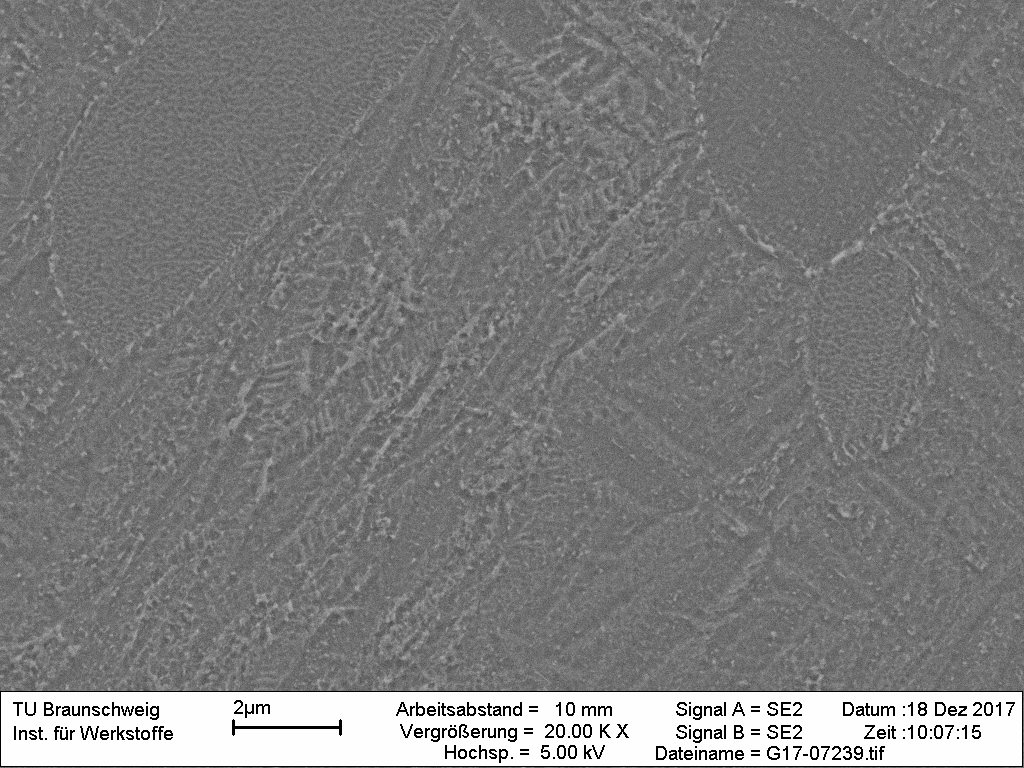
\includegraphics[width=0.66\textwidth]{Bilder/REM950C1hWQ520C24hAC.png}
\caption{REM Aufnahme: 950°C und 24 Stunden Alterung}
\label{REM 950C 24h}
\end{figure}

\chapter{Festigkeitssteigernde Mechanismen}
Dieses Kapitel beschäftigt sich mit der Frage, welche Mechanismen bei der Festigkeitssteigerung von Bedeutung sind. Die einzelnen Wärmebehandlungsschritte werden diskutiert und verglichen.

In jedem der Ansätze ging es um Festigkeitssteigerung durch eine erhöhte Grenzflächendichte. Die Versetzungen können bei einer großen Grenzflächendichte nur unter hohem Energieaufwand durch das Bauteil wandern. So entsteht eine hohe Festigkeit.
\section{Alterung des Martensits}
In der in Abschnitt \ref{Festigkeitssteigerung durch Martensitbildung} behandelten Wärmebehandlung ging es um einen Zerfall des Martensits. Dieser sollte in möglichst kleine Bereiche von Alpha- und Beta-Phase zerfallen. Nur so kann die Grenzflächendichte gegenüber dem Martensit erhöht werden. Der kritische Faktor war hierbei, inwiefern der Martensit zerfällt, während die Vergröberung als festigkeitsverringernder Prozess parallel läuft. Ziel war es, diese konkurrierenden Prozesse so zu steuern, dass ein maximaler Festigkeitsgewinn entsteht. 

Ausgehend von den Ergebnissen der ersten Wärmebehandlung wurde festgestellt, dass ein niedriger Primäralpha-Anteil für eine Festigkeitssteigerung sorgt. Es würde also Sinn ergeben, mit dem mit den geringsten Alpha-Anteil enthaltenen Gefüge die Alterung durchzuführen. Wie bereits erwähnt entscheidet jedoch die Konzentration an Beta stabilisierenden Elementen in der Martensit-Phase über einen festigkeitssteigernden Zerfall. In dem Gefüge mit wenig Primäralpha ist die Konzentration an Beta stabilisierenden Elementen auf Grund des großen Volummenanteils der Beta-Phase geringer als in Gefügen mit viel Primär-Alpha. Dies lässt darauf schließen, dass eine Auslagerung von Proben mit einer geringeren Glühtemperatur zu einer größeren Festigkeitssteigerung führt. Die Ergebnisse der Härteprüfungen zeigen genau den Fall. Proben mit einer Glühtemperatur von 970°C haben keine Festigkeitssteigerung erfahren, während die Proben mit einer Glühtemperatur von 950°C deutliche Festigkeitssteigerungen zeigen. So wird die am Anfang aufgestellte These bestätigt, dass für höhere Konzentrationen an Beta stabilisierenden Elementen eine Festigkeitssteigerung bei einer Alterung resultiert. 

Werden die Gefügebilder betrachtet, lässt sich das Ergebnis erklären. Für die Glühtemperaturen sind unterschiedliche Gefüge entstanden. Bei der Auslagerung von einer Glühtemperatur von 970°C zeigt sich ein Zerfall des Martensits. Die ehemaligen Nadeln sind an vielen Stellen unterbrochen und es hat sich sekundäre Alpha- und Beta-Phase gebildet. Dieser Effekt ist bei der Haltezeit von acht Stunden noch stärker ausgebildet. Es ist allerdings auch zu beobachten, dass noch einige Nadeln unverändert vorliegen. Dies spricht für eine zu niedrige Haltezeit, da die Nadeln bei steigender Haltezeit eher zerfallen als bei einer kürzeren. Bei längeren Haltezeiten ist aber auch der konkurrierende Prozess stärker ausgeprägt. Bereits nach acht Stunden ist eine starke Vergröberung der Platten zu erkennen. Eine noch längere Haltezeit würde zu einem noch größeren Wachstum dieser Platten führen, sodass sich die Grenzflächendichte verringert und so die Festigkeit abnimmt. Eine Festigkeitssteigerung durch den Zerfall des verbleibenden Martensits ist also unwahrscheinlich, da die Vergröberung als Nebenprozess vorliegt. So ist auch die nicht vorhandene Festigkeitssteigerung zu erkären. Der Zerfall des Martensits liegt zwar vor und führt zu einer größeren Grenzflächendichte. Aber gleichzeitig resultiert durch die Vergröberung eine Abnahme der Grenzflächendichte. Es lässt sich also schließen, dass die beiden Prozesse aufgrund der konstanten Härtewerte in gleichen Maßen aufgetreten sind. 

Bei der Auslagerung von einer Glühtemperatur von 950°C zeigt sich ein anderes Ergebnis. Die Härteprüfungen zeigen, dass aufgrund der Auslagerung eine Härtesteigerung von circa 3\%  resultiert ist. Bei einer  Analyse der Gefügebilder dieser Proben werden die Unterschiede gegenüber den Proben mit einer Glühtemperatur von 970°C sichtbar. Bei einem Vergleich der Gefügebilder bei gleicher Haltezeit fällt auf, das die Nadeln bei der niedrigeren Glühtemperatur einen höheren Teilungsgrad besitzen. Außerdem sind die Nadeln nicht so grob geworden, wie die der hohen Temperatur. Die Aufteilung der Nadeln in kleine Bereiche erklärt die Festigkeitssteigerung der ausgelagerten Proben. Die Grenzflächendichte wird dadurch stark erhöht und so ist eine Ausbreitung der Versetzungen nur mit einem großen Energieaufwand möglich. 

Allerdings ist auch bei der niedrigeren Temperatur das Martensit-Gefüge noch deutlich zu erkennen. Bei einer Haltezeit von 24 Stunden ist der Martensit jedoch vollständig zerfallen. Die entstandene Beta-Phase ist in den Gefügebildern als helle Bereiche zu erkennen. Innerhalb der entstandenen Beta-Phase hat sich auch Alpha-Phase gebildet. Diese ist durch die dunklen Bereiche zu erkennen. Die Martensitnadeln haben sich also so geteilt, dass die entstandenen Phasen immer abwechselnd vorliegen. So entsteht im Verhältnis zum nicht ausgelagerten Gefüge ein Gefüge mit mehr Grenzflächen, was zu der Festigkeitszunahme führt.

Der Martensit ist wegen der Instabilität der Phase zerfallen. Je mehr Beta stabilisierende Elemente der Martensit enthält, desto eher zerfällt dieser nach Alpha- und Beta-Phase. Dadurch ist auch der Zerfall bei der niedrigeren Glühtemperatur stärker ausgeprägt als der der hohen Temperaturen. Der konkurrierende Prozess ist bei beiden Ausgangstemperaturen aufgetreten. Die Vergröberung hatte jedoch weniger Einfluss auf die Probe mit einer Glühtemperatur von 950°C, da diese den höheren Teilungsgrad der Nadeln besitzt. Ein Wachstum dieser Bereiche würde zwar zu einer Festigkeitsabnahme führen, hat jedoch nicht so einen negativen Einfluss wie eine Verbreiterung der noch vorhandenen Martensitnadeln bei einer von einer Glühtemperatur von 970°C ausgehenden Alterung.

Abschließend ist die Wärmebehandlung so gelaufen wie erwartet. Das Martensit ist unabhängig von dessen Primäralpha-Anteil zerfallen. Aufgrund der niedrigen Konzentration an Beta stabilisierenden Elementen hat jedoch der Zerfall des Martensits bei einem Glühvorgang von 970°C keine festigkeitssteigernde Wirkung. Dies liegt an dem konkurrierenden Prozess, der zu einer Festigkeitsabnahme führt. Die Probe mit einer Glühtemperatur von 950°C konnte hingegen eine deutliche Steigerung der Festigkeit aufweisen. Hier ist das Verhältnis der Bildung von sekundärer Alpha- und Beta-Phase gegenüber der Vergröberung so, dass die Bildung der stabilen Phasen überwiegt und so die Festigkeit gesteigert werden kann.

Die Ergebnisse des Zugversuchs zeigen hervorragende mechanische Eigenschaften. Die Steigerung der Festigkeit wurde bereits erläutert. Die hohe Bruchdehnung ergibt sich aus der Duktilität der Probe. Diese ist aufgrund des Zerfalls des Martensits entstanden. Aus langen Nadeln haben sich kleine Bereiche an Alpha- und Beta-Phase gebildet. Die sind deutlich duktiler als die vorher vorhandene Martensit-Phase.
\bibliographystyle{plain}
\bibliography{literatur}
\listoffigures
\listoftables
\end{document}
